% !TEX TS-program = pdflatex
% !TEX encoding = UTF-8 Unicode
% !BIB TS-program = biber
% !BIB program = biber
\documentclass[12pt]{article}
%%% PAGE DIMENSIONS
\usepackage[margin=2.54cm]{geometry}
\usepackage{setspace}
\doublespacing
\geometry{a4paper}
%%% PACKAGES
% \usepackage{caption}
% \usepackage{subcaption}
\usepackage{graphicx} % For better graphics
\usepackage{grffile}
\usepackage{pdfpages} % To insert pdfs into the library
\usepackage{tikz}
\usepackage{wrapfig}
\usepackage{siunitx}
\usepackage{lscape} % Create landscape orientation for tables
\usepackage{longtable}
\usepackage{booktabs} % for much better looking tables
\usepackage{amsmath} % for better maths
\usepackage{paralist} % very flexible & customisable lists (eg. enumerate/itemize, etc.)
\usepackage{verbatim} % adds environment for commenting out blocks of text & for better verbatim
\usepackage{subfig} % make it possible to include more than one captioned figure/table in a single float
\usepackage[framed,numbered]{matlab-prettifier} % enable inserting matlab code.
\usepackage[parfill]{parskip}
%\addtolength{\jot}{1em}
\usepackage{amssymb}
\usepackage{cancel}
\usepackage{color}
\usepackage{listings}
% DECLARATIONS
\DeclareMathOperator*{\argmax}{argmax} % thin space, limits underneath in displays
% STYLE FORMATTING
\usepackage{xcolor}
\definecolor{codegreen}{rgb}{0,0.6,0}
\definecolor{codegray}{rgb}{0.5,0.5,0.5}
\definecolor{codepurple}{rgb}{0.58,0,0.82}
\definecolor{backcolour}{rgb}{0.95,0.95,0.92}
\lstdefinestyle{mystyle}{
    backgroundcolor=\color{backcolour},   
    commentstyle=\color{codegreen},
    keywordstyle=\color{magenta},
    numberstyle=\tiny\color{codegray},
    stringstyle=\color{codepurple},
    basicstyle=\ttfamily\footnotesize,
    breakatwhitespace=false,         
    breaklines=true,                 
    captionpos=b,                    
    keepspaces=true,                 
    numbers=left,                    
    numbersep=5pt,                  
    showspaces=false,                
    showstringspaces=false,
    showtabs=false,                  
    tabsize=2}
\lstset{style=mystyle}
\usepackage{multicol}
\usepackage{float}
% REFERENCES
\usepackage[backend=biber,style = apa]{biblatex}
\bibliography{sources}
%%% HEADERS & FOOTERS
\usepackage{fancyhdr} % This should be set AFTER setting up the page geometry
\setlength{\headheight}{15pt}
\pagestyle{fancy} % options: empty , plain , fancy
\renewcommand{\headrulewidth}{0pt} % customize the layout...
\lhead{University of Auckland}\chead{Finance 788}\rhead{Connor McDowall}
\lfoot{}\cfoot{\thepage}\rfoot{}
%%% SECTION TITLE APPEARANCE
\usepackage{sectsty}
%%% TABLE OF CONTENTS APPEARANCE
\usepackage[nottoc,notlof,notlot]{tocbibind} % Put the bibliography in the ToC
\usepackage[titles,subfigure]{tocloft} % Alter the style of the Table of Contents
\renewcommand{\cftsecfont}{\rmfamily\mdseries\upshape}
\renewcommand{\cftsecpagefont}{\rmfamily\mdseries\upshape} % No bold!
%%% HYPERLINKING
\usepackage{hyperref}
%%% DOCUMENT
\begin{document}
%%% NEW COMMANDS
\newcommand{\listequationsname}{List of Equations}
\newlistof{myequations}{equ}{\listequationsname}
\newcommand{\myequations}[1]{%
\addcontentsline{equ}{myequations}{\protect\numberline{\theequation}#1}\par}
\newcommand\numberthis{\addtocounter{equation}{1}\tag{\theequation}}
%%% TITLE PAGE
\begin{titlepage}
	\newcommand{\HRule}{\rule{\linewidth}{0.5mm}} % Defines a new command for horizontal lines, change thickness here
	
	\center
	
	%------------------------------------------------
	%	Headings
	%------------------------------------------------
	
	\textsc{\LARGE }\\[1.5cm] % Main heading such as the name of your university/college
	
	\textsc{\Large University of Auckland\\Department of Accounting \& Finance}\\[0.5cm] % Major heading such as course name
	
	%------------------------------------------------
	%	Title
	%------------------------------------------------
	
	\HRule\\[0.5cm]
	
	{\huge\bfseries Neural Networks: A New Frontier for Asset Pricing}\\[0.4cm] % Title of your document
	
	\HRule\\[0.5cm]
	
	%------------------------------------------------
	%	Author(s)
	%------------------------------------------------
	
	{\large\textit{A research essay presented in part fulfilment of the \\ requirements for the degree of Bachelor of Commerce \\ (Honours) in the Department of Accounting and Finance \\ at The University of Auckland}}\\[0.5cm]
	{\large\textit{Author: Connor McDowall \\Supervisor: Dr Paul Geertsema}}\\
	%------------------------------------------------
	%	Date
	%------------------------------------------------
	
	\vfill\vfill\vfill % Position the date 3/4 down the remaining page
	
	{\large\today} % Date, change the \today to a set date if you want to be precise
	 
	%----------------------------------------------------------------------------------------
	
	\vfill % Push the date up 1/4 of the remaining page
\end{titlepage}
\newpage
\tableofcontents
\listoffigures
\listoftables
\listofmyequations
\newpage
\section{Acknowledgements}
\begin{center}
	\textbf{Paul Geertsema}
\end{center}
\newpage
\section{Abstract}
\newpage
\section{Introduction}
\newpage
\section{Research Question(s)}
\section{Motivation(s)}
\section{Literature Review}\label{LR}
Overview of literature in asset pricing (761/751), ML application, factor pricing - very brief, 12pt, double spaced,
\subsection{Asset Pricing}
\subsection{Machine Learning}
Convexity is an important concept in optimisation
Monotonic ranking
\subsection{Machine Learning}
A couple of recent publications highlight the increased application of machine learning algorithms in financial contexts.
\cite{corporate-culture}
Gu et al (\citeyear{eapvml}) explore the comparative use of machine learning in empirical asset pricing.
\subsection{Data}
\section{Theory}
\subsection{Modelling, Loss, and Optimisation}\label{sec:mlo}
We summarize the theory surrounding predictive modelling, loss functions, and optimisation algorithms.
These functions train models by comparing predictions to realized observations using optimisation algorithms to minimize the loss function.
We examine a linear model as our predictive model (\ref{lm}).
Mean square error (\ref{mse}) and Gradient Descent (GD) are basic examples of a loss function and optimisation algorithm, respectively.
\begin{align*}
	\hat{y} &= mx_i + b \numberthis \label{lm}\\
	f(y,(mx_{i} + b)) &= \frac{1}{n} \sum_{i=1}^{n}(y_i - (mx_{i} + b))^{2} \numberthis \label{mse}
\end{align*}
Firstly, gradient descent takes the partial derivatives of the loss function, with the respect to the parameters in our predictive model.
In our example, equations \ref{pdmsem} and \ref{pdmseb} are the partial derivatives for the mean square error loss function.
\begin{align*}
	\frac{\partial f(y,(mx_{i} + b)}{ \partial m} &= \frac{1}{n} \sum_{i=1}^{n}-2x_{i}(y_i - (mx_{i} + b))^{2} \numberthis \label{pdmsem}\\
	\frac{\partial f(y,(mx_{i} + b)}{ \partial b} &= \frac{1}{n} \sum_{i=1}^{n}-2(y_i - (mx_{i} + b))^{2} \numberthis \label{pdmseb}
\end{align*}
Secondly, the algorithm explores epochs, using a learning rate to update parameters to move in the opposite directions of the partial derivatives until settling in a local minima.
This extrema is the optimisation of the loss function, quantifying the accuracy of the predicative model.
Ordinary Least Squares (OLS) regressions is an extension of the linear model prevalent in asset pricing.
\subsection{Ordinary Least Squares (OLS)}\label{ols}
The OLS regression is the most prominent statistical model in asset pricing theory.
Rosenfeld (\citeyear{olsmf}) summarises OLS.
The composition of the true OLS (\ref{true-ols}) model includes four components.
Firstly, \textbf{X}, an n x k matrix of k independent variables for n observations.
Secondly, \textbf{y}, an n x 1 vector of observation on the dependent variable.
Thirdly, \textbf{$\epsilon$}, an n x 1 vector of unexplained error.
Lastly, $\theta$, a k x 1 vector of parameters to be estimated.
\begin{align*}
	y &= X\theta + \epsilon \numberthis \label{true-ols}
\end{align*}
\subsubsection{Estimation Criteria}
The criteria to obtain the parameter estimate ($\hat{\theta}$) relies on the minimisation of the sum of squared residuals (\ref{ssr}).
We highlight the observed residuals (e) are distinct from unexplained disturbances ($\epsilon$).
Equation \ref{res} derives residuals by taking the difference between observations based on parameter estimates.
\begin{align*}
	\sum & e_i^2  \numberthis \label{ssr}\\
	e = y & - X \hat{\theta} \numberthis \label{res}
\end{align*}
Expanding the quadratic $e^{T}e$ after substituting in equation \ref{res} leads to the alternative expression of the sum of squared residuals in equation \ref{ssrm}.
Minimizing the sum of square residuals requires taking the partial derivative of equation \ref{ssrm} with respect to the estimated parameters (equation) using matrix differentiation (\ref{ssrmd}).
It is imperative X has full rank where all vectors in the matrix are linearly independent, validating both the presence of a positive definite matrix and minimum.
\begin{align*}
	e^{T}e &= y^{T}y - 2\hat{\theta}^{T}X^{T}y + \hat{\theta}^{T}X^{T}\hat{\theta}X \numberthis \label{ssrm}\\
	\frac{\partial e^{T}e}{\partial \hat{\theta}} &= - 2X^{T}y + 2X^{T}X\hat{\theta} =0 \numberthis \label{ssrmd}
\end{align*}
We find the expression for the Ordinary Least Squares (OLS) estimator (\ref{OLSD}) after rearranging equation \ref{ssrmd} to normal form, utilizing inverse matrices to form identity matrices, and simplifying.
\begin{align*}
	2X^{T}X\hat{\theta} &= 2X^{T}y \\
	(X^{T}X)^{-1}(X^{T}X)\hat{\theta} &= (X^{T}X)^{-1}X^{T}y \\
	I\hat{\theta} &= (X^{T}X)^{-1}X^{T}y \\
	\hat{\theta} &= (X^{T}X)^{-1}(X^{T}y) \numberthis \label{OLSD}\\
\end{align*}
Therefore, we can use the OLS estimator to make predictions with OLS (\ref{OLS}).
\begin{align*}
	\hat{y} &= X^{T} \hat{\theta} \numberthis \label{OLS}
\end{align*}
\subsubsection{Properties of OLS Estimators}
There are six key properties in addition to the satisfaction in minimizing the summation of squared residuals.
\begin{enumerate}
	\item The residuals are uncorrelated with the observed values of X i.e., $X^{T}e=0$.
	\item The sum of the residuals is zero i.e., $\sum e_i=0$.
	\item The sample mean of the residuals is zero i.e., $\bar{e} = \frac{\sum e_i}{n} = 0$.
	\item The regression hyperplane passes through the means of observed values i.e., $\frac{e} = \frac{y - X\theta}{n} = 0$. Since $\bar{e} = 0$ assumed, it is implied $\bar{y}=\bar{x}\bar{\theta}$.
	\item The residuals are uncorrelated with the predicted y i.e., $\hat{y} = X\hat{\theta}$, $\hat{y}^{T}e = (X\hat{\beta})^{T}e = b^{T}X^{T}e = 0$ 
	\item The mean of $\hat{y}$ for the sample will equal the mean of the y.
\end{enumerate}
\subsubsection{The Gauss-Markov Theorem}
However, OLS makes Gauss-Markov assumptions about the true model to make inferences regarding $\beta$ from $\hat{\beta}$.
The intention of the Gauss-Markov Theorem, conditional on the below assumptions, states the OLS estimator is the best linear, unbiased, and efficient estimator: 
\begin{align*}
	y &= x\beta + \epsilon\\
	E[\epsilon|X] &= 0 \numberthis \label{gma3}\\
	E(\epsilon \epsilon^{T}|X) &= \Omega = \sigma^{2}I \numberthis \label{gma4}\\
	\epsilon &| X ~ N[0,\sigma^{T}I] \text{ (hypothesis testing)}
\end{align*}
\begin{itemize}
	\item X is an n x k matrix of full rank
	\item X must be generated randomly, or fixed, by a mechanism uncorrelated to disturbances.
\end{itemize}
Equation \ref{gma3} implies $E(y) = X\beta$ as no observations of the independent variables convey any information about the expected values of the disturbances.
Equation \ref{gma4} captures homoskedasticity and no autocorrelation assumptions.
Additionally,
The theory underlying Ordinary Least Squares informs the common practice in minimising of the sum of least squares when evaluating prediction performance.
The mathematical tractability, in accordance with the aforementioned assumption, frame our thinking surrounding the derivation of custom loss functions.
\subsection{Artificial Neural Networks (ANN)}
\subsubsection{Multi Layer Perceptron (MLP)}\label{mlp-math}
Artificial Neural Nets (ANN) are versatile, powerful, and scalable.
They sit at the heart of deep learning as frequently outperform other machine learning algorithms on large and complex problems.
This research proposal suggests implementing two sets of multi-layer perceptron, a form of ANN, to predict investment decisions and exit opportunities from investment criteria.
A linear threshold unit (LTU) feeds the weighted sum of input values ($z=\textbf{w}^{T} \cdot \textbf{x}$) into a step function ($h_{w}(\textbf{x})=step(z)$).
A perceptron is a single layer of LTUs where each LTU is connected to every input.
Perceptrons are suitable for classification as output the positive investment decision or exit opportunity if a threshold is met.
Perceptrons utilize a training algorithm assessing the strength of connections between perceptrons while considering errors.
A perceptron is fed one training instance at a time, making predictions for each instance.
For every output LTU that produced a wrong prediction, it re-enforces the connection weights using the perception learning rule (\ref{mlp-plr}) from the inputs that would have contributed to the right prediction.
A Multi Layer Perceptron is composed of one LTU input layer, multiple LTU hidden layers and an output LTU layer.
The step functions in each LTU are replaced by a logistic or ReLU function ($\sigma(z)=\frac{1}{1+ exp(-z)}$ or $ReLU(z) = max(0,z)$ respectively) to enable gradient descent for optimisation.
A shared softmax function replaces the individual activation functions in the output layer to enable exclusive classification.
In this instance, the classification of investment decisions, or exit opportunties, from investment criteria.
Tensorflow's DNNClassifier function facilitates the implementation of MLPs in this proposal.
\begin{align}
	w_{i,j}^{\text{next step}} &= w_{i,j} + \eta (\hat{y}_j - y_j)x_i \numberthis \label{mlp-plr}
\end{align}
Where
\begin{itemize}
	\item $w_{i,j}$ is the connection weights between the ith input neuron and the jth output neuron. 
	\item $x_i$ is the ith input value of the current training instance.
	\item $\hat{y}_{j}$ is the output of the jth output neuron for the current training instance.
	\item $y_{j}$ is the output of the jth output neuron for the current training instance.
	\item $\eta$ is the rate.
\end{itemize}
\subsection{Hypothesis}
\textbf{Include examples on the minimisation of sum of the square errors does not contribute to maximising returns}
\section{Model}
\textbf{Insert model configuration}
Example of the whole set
\begin{align*}

\end{align*}
\subsection{Configuration}
\section{Methodology}
\subsection{Data}
Hou et al., (\citeyear{hou2020replicating}) use an extensive data library to assess 452 anomalies across anomalies literature.
Their analysis informs which abnormalities drive the cross section of expected returns. 
Most abnormalities fail under current standards of empirical finance when using a single hurdle test of absolute t-stat greater or equal to 1.96.
Firstly, the paper finds economic fundamentals take precedence over trading frictions in explanatory power, statistical and economic significance.
Secondly, micro-caps account for anomalies disproportionately, leading to NYSE breakpoints, value-weighted returns in both portfolio sorts and cross-sectional regressions with weighted least squares. 
Lastly, arguments in improving anomalies literature credibility follow a closer alignment to economic theory as the field persists to be statistical in nature.
Overall, capital market efficiency is higher than expected.
Jensen et al., \citeyear{jensen2021there} use the above dataset to explore hierarchial bayesian models of alphas emphasising the joint behaviours of factors, 
and provide an alternative multiple testing adjustment, more powerful than common methods.
Jensen et al., adapt the global dataset to focus only on one-month holding periods for all factors, only include most recent accounting data (quarterly or annually) and add 15 new factors.
The exhaustive nature and accessibility of the global dataset makes it well-suited for exploring optimisation functions in neural-network construction.
\subsection{Limitations}
\subsection{Summary Statistics}
\section{Methodology}
\subsection{Target Variable}
\subsection{Google Cloud Platform}
\subsubsection{Configuration}
\subsubsection{Limitations}
\subsection{Tensorflow}
\subsubsection{Automatic Differientiation}
\subsection{Loss Functions \& Performance Metrics}
Table \ref{hpt} emphasises the separation between training and validation datasets.
	\begin{table}[H]
		\centering
		\begin{tabular}{||c|c|c|c||}
			\hline
			Variable & Description & $ MSE(y,\hat{y}) $ & $ HP(y,\hat{y}) $\\ [0.5ex]
			\hline
			&&&\\
			$\theta$ & Estimation& $ \hat{\theta}_{MSE}$& $ \hat{\theta}_{HP}$ \\ [0.5ex]
			& Training & & \\
			\hline
			&&&\\
			$\lambda$ & Validation & $\hat{\lambda}_{MSE}$ & $\hat{\lambda}_{HP}$\\ [1.0ex]
			\hline
		\end{tabular}
	\caption{Objective (MSE: Mean Square Error, HP: Hedge Portfolio)}
	\label{hpt}
\end{table}
\subsubsection{Mean Square Error (MSE)}
Section \ref{sec:mlo} outlines advantages to Ordinary Least Squares.
Subsequently, MSE serves as a baseline for loss function and performance metric comparisons.
The following function (\ref{mself}) and partial derivative (\ref{pdmself}) describe Tensorflows's Mean Square Error implementation, both from in-built and custom contexts. 
Python classes describe equation \ref{mself} to enable Tensorflow's automatic differentiation capabilities, approximating the partial derivatives of the loss function (\ref{pdmself}) with numerical methods.
Please note the use of Hadamard exponentiation ($x^{\circ n}$) as an element-wise operation.
\begin{align*}
	f(y, X^{T} \hat{\theta}) &= \frac{\vec{1}}{\vec{1}^{T}\vec{1}} (y - X^{T}\hat{\theta})^{\circ 2} \numberthis \label{mself}\\
	\frac{\partial f(y, X^{T} \hat{\theta})}{ \partial \hat{\theta}} &= \frac{\vec{1}}{\vec{1}^{T}\vec{1}} (-2(y-X{T} \hat{\theta})^{\circ 1}) \numberthis \label{pdmself}\\
\end{align*}
\subsubsection{Hedge Portfolio}
Hedge portfolios rely on monotonic ranking functions for optimisation as their monotonic nature preserves or reverses a given ordered set.
The analysis cross-section of one-month lead portfolio excess returns using monotonic functions 
\begin{align}
	R(y_{i,t}) \numberthis \label{ranking-function}
\end{align}
The ranking function (R($y_{i,t}$)) and thresholds (u,v) form subsets of long and short portfolios.
Long (L) or Short (S) sets include excess returns conditioned on the associated monotonic ranking given a threshold, bound by the cardinality of the excess return vector ($|y|$).
The subsequent truth sets mathematically express aforementioned time-series hedge portfolios.
\begin{align*}
	L &= \{ y_{i,t} | R(y_{i,t})\leq u\}\\
	S &= \{ y_{i,t} | R(y_{i,t})\geq v\}\\
	0 & < u \leq |y|\\
	0 & < v \leq |y|\\
	u & < v
\end{align*}
Equation \ref{htls} describes hedge portfolio lead excess returns ($H_t$) at a given time (t).
\begin{align}
	H_t &= \frac{1}{|L|}\sum_{i\epsilon L} y_{i,t} - \frac{1}{|S|}\sum_{i\epsilon S} y_{i,t} \label{htls}
\end{align}
Figure \ref{fig:mrf}) illustrates an approximate linear monotonic ranking function with a sample of 100 uniformly distributed excess returns  between -10\% and 10\%.
Boundary conditions u and v are set to 20 and 80 , respectively.
Subsequently, excess returns above (below) the green (blue) dotted line belong to the long (L) (short (S)) set. 
\begin{figure}[H]
    \centering 
    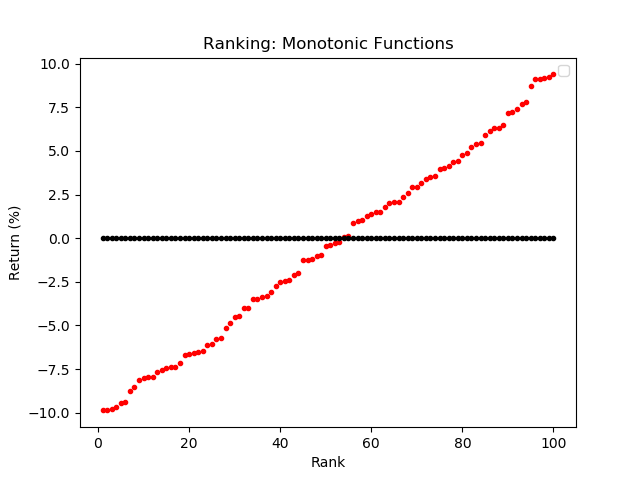
\includegraphics[width=\textwidth]{{/Users/connor/Google Drive/Documents/University/Courses/2020-21/Finance 788/finance-honours/results/plots/monotonic-ranking}.png}
    \caption{Approximate Linear Monotonic Ranking Function}
    \label{fig:mrf}
\end{figure}
The permutations in monotonic ranking functions, and subsequent hedge portfolios, are endless. 
This research essay develops a monotonic ranking function proportionally weighting one month lead excess returns (\ref{w1}).
Therefore, equation \ref{pwlf} defines the loss function.
\begin{align*}
	R(\hat{y}) &= W \numberthis \label{w1}\\
	W&:= \frac{\hat{y}}{\vec{\textbf{1}}\hat{y}}\\
	\hat{y} &= X^{T} \hat{\theta}\\
	f_{\hat{\theta}}(X) &= (\frac{X^{T} \hat{\theta}}{\vec{\textbf{1}}X^{T} \hat{\theta}})^\top X^{T} \hat{\theta} \numberthis \label{pwlf}
\end{align*}
The above loss function is differentiable using symbolic mathematic as shown in equation \ref{pdewlf}.
\begin{align*}
	\frac{\partial f_{\hat{\theta}}(X)}{\partial \hat{\theta}} &= \frac{\partial ((\frac{X^{T} \hat{\theta}}{\vec{\textbf{1}}X^{T} \hat{\theta}})^\top X^{T} \hat{\theta})}{\partial \hat{\theta}} \\
	\frac{\partial (f_{\hat{\theta}}(X))}{\partial \hat{\theta}}  &= \frac{1}{(\hat{\theta}^\top X \vec{1})} X X^\top \hat{\theta} +\frac{1}{\vec{1}X^\top \hat{\theta}} XX^\top \hat{\theta} -\frac{1}{(\hat{\theta}^\top X \vec{1})^{2}} \hat{\theta}^\top XX^\top \hat{\theta} X \vec{1} \numberthis \label{pdewlf}
\end{align*}
Our research
Subsection \ref{sec:mlo} explains the theory supporting loss minimisation.
Applying gradient descent methods to the product of  the loss function and scaler of -1 transforms the minimisation to maximisation.
This transformation leads to finding the argmax of maximisation function with respect to $\hat{\theta}$ (\ref{argmax}).
The aforementioned transformation is simply and suitable for exploration in the context of the research intent.
More sophisticated methods exist for maximisation such as reinforcement learning (\ref{rifml}).
\begin{align*}
	\argmax_{\hat{\theta}} &: (\frac{X^{T} \hat{\theta}}{\vec{\textbf{1}}X^{T} \hat{\theta}})^\top X^{T} \hat{\theta} \numberthis \label{argmax}
\end{align*}
Conventional asset pricing methodologies persist in academic literature.
Subsequently, this research essay uses the Hedge Portfolio Mean (\ref{hm})), Capital Asset Pricing Model (\ref{hcapm}), 
Fama-French Three Factor Model (\ref{hff3}), and Fama-French Five Factor Model (\ref{hff5}) as performance metrics for each loss function.
The use of the Capital Asset Pricing Model (CAPM) persists, regardless of the identifiable shortcomings in market proxies and empirical failings invalidating use (\cite{fama2004capital}).
Nonetheless, this research essay uses the model as a performance metric for comparative purposes.
\begin{align*}
	R_{i,t} - R_{f,t} &= \alpha_{i,t} + \beta_{i,t}(R_{M,t}-R_{f,t}) \numberthis \label{capm}
\end{align*}
E. Fama and K. French (\citeyear{eugene1992cross}) validate the explanatory power of size and value (book-to-market) factors
in their ability to capture the cross-sectional variation in average stock returns, in association with market risk, size, leverage, book-to-market, and earnings-price ratios.
This combination of factors is known as the Fama-French Three Factor Model (FF3). 
E. Fama and J. MacBeth developed the Fama-MacBeth regressions, a two-stage methodology to deriving factor prices.
First,
\begin{align*}
	H_{\mu} &=1 \numberthis \label{hm}\\
	H_{CAPM} &= 1 \numberthis \label{hcapm}\\
	H_{FF3} &= 1 \numberthis \label{hff3}\\
	H_{FF5} &= 1 \numberthis \label{hff5}
\end{align*}
Fama-French Five Factor Model (FF5) continues to inform asset pricing E. Fama \& K. French produce \cite{fama2004capital}
\subsubsection{Sharpe Ratio}
Nobel Laurette William F. Sharpe (\citeyear{sharpe1994sharpe}) introduced the Sharpe Ratio (\ref{sr}) as a measure for risk-adjusted returns
where $\mathop{\mathbb{E}} [R_a - R_f]$ is the expectation for excess returns and $\sigma(R_a)$ is the standard deviation of excess returns.
\begin{align*}
	SR &= \mathop{\mathbb{E}} \frac{[R_a - R_f]}{\sigma(R_a)} \numberthis \label{sr}\\
	\sigma &= \sqrt{\sum_{i=1}^{n}}\frac{(R_a) - \bar{R_a})^2}{n}
\end{align*}
The matrix notation for the Sharpe Ratio loss function () follows:
\begin{align*}
	SR &= 1 \numberthis \label{srlf}
	\partial SR
\end{align*}
\subsubsection{Information Ratio}
The Information Ratio (IR) is another risk-return measure (\ref{ir}), evaluating the performance of a portfolio compared to a selected benchmark e.g., an exchange traded fund.
$\mathop{\mathbb{E}} [R_a - R_b]$ is the excess return on the benchmark. $\sigma(R_a - R_b)$ is the standard deviation of the difference between the portfolio and benchmark known as the tracking error.
\begin{align*}
	IR &= \mathop{\mathbb{E}} \frac{[R_a - R_b]}{\sigma(R_a - R_b)} \numberthis \label{sr}\\
\end{align*}
% Show the embedded class structure within this section.
\subsection{Reinforcement learning} \label{rifml}
\subsubsection{Dynamic Programming}
\subsubsection{Bellman's Algorithm}
\subsubsection{Q-Learning}
\newpage
\section{Results}
\section{Discussion}
\section{Contributions}
\section{Conclusion}
\newpage
\begin{landscape}
\section{Appendix}
\subsection{Tables and Charts}
\setlength{\tabcolsep}{2pt}
\begin{longtable}{|l|r|r|r|r|r|r|r|r|}
\toprule
{} &      count &          mean &           std &         min &           25\% &           50\% &           75\% &           max \\
\midrule
\endhead
permno                  &  2739928.0 &  5.405281e+04 &  2.782267e+04 &  10000.0000 &  2.651800e+04 &  5.715400e+04 &  8.018600e+04 &  9.343600e+04 \\
permco                  &  2739928.0 &  1.843974e+04 &  1.402881e+04 &      3.0000 &  7.702000e+03 &  1.640850e+04 &  2.321000e+04 &  5.766700e+04 \\
crsp\_shrcd              &  2739928.0 &  1.089520e+01 &  4.571000e-01 &     10.0000 &  1.100000e+01 &  1.100000e+01 &  1.100000e+01 &  1.200000e+01 \\
crsp\_exchcd             &  2739928.0 &  2.127400e+00 &  9.343000e-01 &      1.0000 &  1.000000e+00 &  3.000000e+00 &  3.000000e+00 &  3.000000e+00 \\
sic                     &  2692217.0 &  4.605936e+03 &  1.921398e+03 &    100.0000 &  3.271000e+03 &  4.011000e+03 &  6.036000e+03 &  9.999000e+03 \\
ff49                    &  2674304.0 &  3.037380e+01 &  1.341740e+01 &      1.0000 &  1.800000e+01 &  3.400000e+01 &  4.300000e+01 &  4.900000e+01 \\
adjfct                  &  2739928.0 &  2.838700e+00 &  1.267170e+01 &      0.0000 &  1.000000e+00 &  1.000000e+00 &  2.000000e+00 &  1.215000e+03 \\
shares                  &  2739928.0 &  6.078630e+01 &  2.852566e+02 &      0.0830 &  4.399000e+00 &  1.251900e+01 &  3.808200e+01 &  2.920640e+04 \\
me                      &  2739928.0 &  2.241254e+03 &  1.473073e+04 &      1.1708 &  4.367020e+01 &  1.565628e+02 &  7.167608e+02 &  2.255969e+06 \\
me\_company              &  2739928.0 &  2.283180e+03 &  1.527340e+04 &      1.1708 &  4.387450e+01 &  1.574086e+02 &  7.211363e+02 &  2.255969e+06 \\
prc                     &  2739928.0 &  2.876220e+01 &  6.488772e+02 &      0.0078 &  7.875000e+00 &  1.612500e+01 &  2.912500e+01 &  1.416000e+05 \\
prc\_local               &  2739928.0 &  2.876220e+01 &  6.488772e+02 &      0.0078 &  7.875000e+00 &  1.612500e+01 &  2.912500e+01 &  1.416000e+05 \\
dolvol                  &  2580622.0 &  3.282292e+08 &  2.520900e+09 &      0.0000 &  1.070786e+06 &  7.165154e+06 &  7.076108e+07 &  8.441730e+11 \\
ret                     &  2719460.0 &  1.640000e-02 &  1.672000e-01 &     -1.0000 & -5.880000e-02 &  4.100000e-03 &  7.410000e-02 &  2.400000e+01 \\
ret\_local               &  2719460.0 &  1.640000e-02 &  1.672000e-01 &     -1.0000 & -5.880000e-02 &  4.100000e-03 &  7.410000e-02 &  2.400000e+01 \\
ret\_exc                 &  2719460.0 &  1.270000e-02 &  1.673000e-01 &     -1.0068 & -6.250000e-02 &  7.000000e-04 &  7.060000e-02 &  2.399690e+01 \\
ret\_lag\_dif             &  2739928.0 &  1.000000e+00 &  0.000000e+00 &      1.0000 &  1.000000e+00 &  1.000000e+00 &  1.000000e+00 &  1.000000e+00 \\
ret\_exc\_lead1m          &  2732542.0 &  6.400000e-03 &  1.559000e-01 &     -1.0113 & -6.560000e-02 & -1.800000e-03 &  6.710000e-02 &  1.988170e+01 \\
market\_equity\_rank\_x    &  2739928.0 &  5.982920e+01 &  2.380660e+01 &      1.0000 &  4.000000e+01 &  6.000000e+01 &  8.000000e+01 &  9.950000e+01 \\
enterprise\_value\_rank\_x &  2480615.0 &  5.845440e+01 &  2.501660e+01 &      1.0000 &  3.800000e+01 &  5.900000e+01 &  8.000000e+01 &  9.950000e+01 \\
book\_equity\_rank\_x      &  2452453.0 &  5.800700e+01 &  2.593820e+01 &      1.0000 &  3.800000e+01 &  5.900000e+01 &  8.000000e+01 &  9.950000e+01 \\
assets\_rank\_x           &  2522907.0 &  5.751850e+01 &  2.635510e+01 &      1.0000 &  3.700000e+01 &  5.900000e+01 &  8.000000e+01 &  9.950000e+01 \\
sales\_rank\_x            &  2509790.0 &  5.691950e+01 &  2.717080e+01 &      1.0000 &  3.600000e+01 &  5.900000e+01 &  8.000000e+01 &  9.950000e+01 \\
net\_income\_rank\_x       &  2517298.0 &  5.581200e+01 &  2.878360e+01 &      1.0000 &  3.300000e+01 &  6.000000e+01 &  8.000000e+01 &  9.950000e+01 \\
bidask\_x                &  2739928.0 &  1.289000e-01 &  3.351000e-01 &      0.0000 &  0.000000e+00 &  0.000000e+00 &  0.000000e+00 &  1.000000e+00 \\
prc\_high\_x              &  2355383.0 &  2.540480e+01 &  2.608370e+01 &      0.1790 &  9.250000e+00 &  1.850000e+01 &  3.300000e+01 &  4.617600e+02 \\
prc\_low\_x               &  2365005.0 &  2.211970e+01 &  2.325750e+01 &      0.0818 &  7.640000e+00 &  1.600000e+01 &  2.880000e+01 &  4.175300e+02 \\
tvol\_x                  &  2580622.0 &  8.316484e+06 &  2.941295e+07 &      0.0000 &  9.875000e+04 &  5.510000e+05 &  3.923700e+06 &  6.485186e+08 \\
div1m\_me\_x              &  2718102.0 &  1.300000e-03 &  3.700000e-03 &      0.0000 &  0.000000e+00 &  0.000000e+00 &  0.000000e+00 &  9.010000e-02 \\
div3m\_me\_x              &  2718121.0 &  4.000000e-03 &  6.000000e-03 &      0.0000 &  0.000000e+00 &  0.000000e+00 &  6.700000e-03 &  1.164000e-01 \\
div6m\_me\_x              &  2660395.0 &  8.100000e-03 &  1.170000e-02 &      0.0000 &  0.000000e+00 &  0.000000e+00 &  1.360000e-02 &  1.472000e-01 \\
div12m\_me\_x             &  2548844.0 &  1.670000e-02 &  2.350000e-02 &      0.0000 &  0.000000e+00 &  3.800000e-03 &  2.780000e-02 &  4.015000e-01 \\
chcsho\_1m\_x             &  2720001.0 &  3.200000e-03 &  2.550000e-02 &     -0.1168 &  0.000000e+00 &  0.000000e+00 &  0.000000e+00 &  1.096800e+00 \\
chcsho\_3m\_x             &  2681179.0 &  1.240000e-02 &  6.180000e-02 &     -0.1424 &  0.000000e+00 &  0.000000e+00 &  3.300000e-03 &  1.686700e+00 \\
chcsho\_6m\_x             &  2624125.0 &  2.810000e-02 &  1.189000e-01 &     -0.1880 &  0.000000e+00 &  9.000000e-04 &  1.070000e-02 &  3.832600e+00 \\
chcsho\_12m\_x            &  2514147.0 &  6.190000e-02 &  2.297000e-01 &     -0.2696 &  0.000000e+00 &  4.700000e-03 &  3.390000e-02 &  8.477000e+00 \\
eqnpo\_1m\_x              &  2718435.0 & -1.500000e-03 &  2.310000e-02 &     -0.6801 & -0.000000e+00 &  0.000000e+00 &  0.000000e+00 &  1.263000e-01 \\
eqnpo\_3m\_x              &  2677912.0 & -6.200000e-03 &  5.200000e-02 &     -0.9973 & -1.800000e-03 &  0.000000e+00 &  8.000000e-03 &  1.696000e-01 \\
eqnpo\_6m\_x              &  2618619.0 & -1.350000e-02 &  8.900000e-02 &     -1.5754 & -7.400000e-03 &  0.000000e+00 &  1.640000e-02 &  2.788000e-01 \\
eqnpo\_12m\_x             &  2504936.0 & -2.670000e-02 &  1.474000e-01 &     -2.2489 & -2.450000e-02 &  0.000000e+00 &  3.340000e-02 &  4.743000e-01 \\
ret\_1\_0\_x               &  2541516.0 &  1.490000e-02 &  1.481000e-01 &     -0.7242 & -6.120000e-02 &  7.900000e-03 &  7.690000e-02 &  2.176500e+00 \\
ret\_2\_0\_x               &  2521767.0 &  2.960000e-02 &  2.125000e-01 &     -0.8327 & -8.110000e-02 &  1.480000e-02 &  1.176000e-01 &  3.342500e+00 \\
ret\_3\_0\_x               &  2503682.0 &  4.400000e-02 &  2.649000e-01 &     -0.8864 & -9.610000e-02 &  2.270000e-02 &  1.506000e-01 &  5.000000e+00 \\
ret\_3\_1\_x               &  2502019.0 &  2.870000e-02 &  2.108000e-01 &     -0.8310 & -8.140000e-02 &  1.440000e-02 &  1.167000e-01 &  3.342500e+00 \\
ret\_6\_0\_x               &  2447794.0 &  8.830000e-02 &  3.970000e-01 &     -0.9396 & -1.267000e-01 &  4.500000e-02 &  2.336000e-01 &  8.555600e+00 \\
ret\_6\_1\_x               &  2446030.0 &  7.230000e-02 &  3.553000e-01 &     -0.9171 & -1.184000e-01 &  3.700000e-02 &  2.059000e-01 &  8.411800e+00 \\
ret\_9\_0\_x               &  2393988.0 &  1.336000e-01 &  5.093000e-01 &     -0.9721 & -1.466000e-01 &  6.750000e-02 &  3.069000e-01 &  9.857100e+00 \\
ret\_9\_1\_x               &  2392087.0 &  1.168000e-01 &  4.700000e-01 &     -0.9555 & -1.414000e-01 &  5.930000e-02 &  2.812000e-01 &  9.273700e+00 \\
ret\_12\_0\_x              &  2341375.0 &  1.813000e-01 &  6.179000e-01 &     -0.9783 & -1.593000e-01 &  9.080000e-02 &  3.773000e-01 &  1.301590e+01 \\
ret\_12\_1\_x              &  2339380.0 &  1.635000e-01 &  5.789000e-01 &     -0.9728 & -1.558000e-01 &  8.200000e-02 &  3.514000e-01 &  1.223080e+01 \\
ret\_12\_7\_x              &  2337747.0 &  7.050000e-02 &  3.478000e-01 &     -0.9055 & -1.163000e-01 &  3.610000e-02 &  2.015000e-01 &  8.509400e+00 \\
ret\_18\_1\_x              &  2239551.0 &  2.625000e-01 &  7.812000e-01 &     -0.9850 & -1.710000e-01 &  1.321000e-01 &  4.926000e-01 &  2.048480e+01 \\
ret\_24\_1\_x              &  2145964.0 &  3.596000e-01 &  9.260000e-01 &     -0.9890 & -1.717000e-01 &  1.837000e-01 &  6.267000e-01 &  1.484620e+01 \\
ret\_24\_12\_x             &  2142652.0 &  1.821000e-01 &  6.037000e-01 &     -0.9678 & -1.493000e-01 &  9.260000e-02 &  3.714000e-01 &  1.345160e+01 \\
ret\_36\_1\_x              &  1976435.0 &  5.673000e-01 &  1.234400e+00 &     -0.9935 & -1.548000e-01 &  2.964000e-01 &  8.916000e-01 &  1.914000e+01 \\
ret\_36\_12\_x             &  1972590.0 &  3.838000e-01 &  9.482000e-01 &     -0.9864 & -1.546000e-01 &  2.006000e-01 &  6.490000e-01 &  1.702520e+01 \\
ret\_48\_12\_x             &  1821582.0 &  5.938000e-01 &  1.256400e+00 &     -0.9918 & -1.358000e-01 &  3.161000e-01 &  9.172000e-01 &  1.811810e+01 \\
ret\_48\_1\_x              &  1826053.0 &  7.976000e-01 &  1.577300e+00 &     -0.9965 & -1.285000e-01 &  4.175000e-01 &  1.176300e+00 &  1.772000e+01 \\
ret\_60\_1\_x              &  1691563.0 &  1.064400e+00 &  2.014800e+00 &     -0.9985 & -9.170000e-02 &  5.486000e-01 &  1.492300e+00 &  2.754720e+01 \\
ret\_60\_12\_x             &  1686573.0 &  8.258000e-01 &  1.611700e+00 &     -0.9960 & -1.096000e-01 &  4.364000e-01 &  1.200000e+00 &  2.063640e+01 \\
ret\_60\_36\_x             &  1680619.0 &  3.857000e-01 &  9.340000e-01 &     -0.9860 & -1.429000e-01 &  2.072000e-01 &  6.479000e-01 &  1.808570e+01 \\
seas\_1\_1an\_x            &  2426517.0 &  1.420000e-02 &  1.421000e-01 &     -0.6705 & -6.040000e-02 &  7.600000e-03 &  7.560000e-02 &  1.823500e+00 \\
seas\_1\_1na\_x            &  1870192.0 &  1.490000e-02 &  4.360000e-02 &     -0.2355 & -7.800000e-03 &  1.280000e-02 &  3.460000e-02 &  3.871000e-01 \\
seas\_2\_5an\_x            &  1599992.0 &  1.520000e-02 &  6.790000e-02 &     -0.2970 & -2.260000e-02 &  1.180000e-02 &  4.810000e-02 &  6.337000e-01 \\
at\_gr1\_x                &  2426455.0 &  2.641000e-01 &  9.239000e-01 &     -0.7398 &  4.800000e-03 &  9.050000e-02 &  2.391000e-01 &  3.163840e+01 \\
ca\_gr1\_x                &  2184566.0 &  3.206000e-01 &  1.336600e+00 &     -0.8313 & -3.830000e-02 &  9.400000e-02 &  2.815000e-01 &  4.636900e+01 \\
nca\_gr1\_x               &  2183067.0 &  3.950000e-01 &  1.682300e+00 &     -0.8737 & -1.530000e-02 &  8.250000e-02 &  2.844000e-01 &  5.781320e+01 \\
lt\_gr1\_x                &  2408077.0 &  3.042000e-01 &  9.791000e-01 &     -0.8021 & -2.990000e-02 &  8.560000e-02 &  2.894000e-01 &  1.783760e+01 \\
cl\_gr1\_x                &  2190296.0 &  2.996000e-01 &  8.898000e-01 &     -0.8494 & -6.490000e-02 &  1.114000e-01 &  3.701000e-01 &  1.634630e+01 \\
ncl\_gr1\_x               &  2075342.0 &  9.926000e-01 &  5.509500e+00 &     -1.0000 & -1.023000e-01 &  3.970000e-02 &  3.376000e-01 &  1.990000e+02 \\
be\_gr1\_x                &  2311345.0 &  3.178000e-01 &  1.301000e+00 &     -0.9166 &  5.900000e-03 &  9.660000e-02 &  2.271000e-01 &  3.373330e+01 \\
debt\_gr1\_x              &  2158693.0 &  7.838000e-01 &  4.707200e+00 &     -1.0000 & -1.456000e-01 &  1.900000e-02 &  3.292000e-01 &  1.090000e+02 \\
sale\_gr1\_x              &  2362404.0 &  2.228000e-01 &  6.711000e-01 &     -0.9960 &  5.000000e-03 &  1.032000e-01 &  2.478000e-01 &  1.370570e+01 \\
cogs\_gr1\_x              &  2358805.0 &  2.142000e-01 &  6.122000e-01 &     -0.9619 & -4.700000e-03 &  1.032000e-01 &  2.613000e-01 &  1.190030e+01 \\
sga\_gr1\_x               &  1997437.0 &  1.844000e-01 &  3.963000e-01 &     -1.0000 &  1.340000e-02 &  1.044000e-01 &  2.389000e-01 &  6.765800e+00 \\
opex\_gr1\_x              &  2387208.0 &  1.949000e-01 &  4.470000e-01 &     -0.7668 &  7.900000e-03 &  1.058000e-01 &  2.505000e-01 &  7.187400e+00 \\
capx\_gr1\_x              &  2147147.0 &  6.016000e-01 &  2.183000e+00 &     -1.3370 & -2.236000e-01 &  1.144000e-01 &  6.251000e-01 &  3.425000e+01 \\
inv\_gr1\_x               &  1910333.0 &  2.595000e-01 &  9.931000e-01 &     -1.0000 & -6.850000e-02 &  8.260000e-02 &  2.909000e-01 &  1.698080e+01 \\
at\_gr3\_x                &  2114339.0 &  9.104000e-01 &  2.670800e+00 &     -0.8797 &  8.870000e-02 &  3.426000e-01 &  8.167000e-01 &  6.899070e+01 \\
ca\_gr3\_x                &  1898998.0 &  9.832000e-01 &  3.187300e+00 &     -0.9099 &  2.890000e-02 &  3.230000e-01 &  8.289000e-01 &  7.748590e+01 \\
nca\_gr3\_x               &  1897746.0 &  1.592100e+00 &  6.786800e+00 &     -0.9628 &  4.280000e-02 &  3.455000e-01 &  1.005000e+00 &  1.792615e+02 \\
lt\_gr3\_x                &  2091277.0 &  1.135900e+00 &  3.376000e+00 &     -0.8936 &  3.580000e-02 &  3.474000e-01 &  9.457000e-01 &  5.633890e+01 \\
cl\_gr3\_x                &  1906078.0 &  9.845000e-01 &  2.656400e+00 &     -0.9194 &  9.000000e-03 &  3.652000e-01 &  9.754000e-01 &  4.535460e+01 \\
ncl\_gr3\_x               &  1803330.0 &  4.168200e+00 &  2.242620e+01 &     -1.0000 & -1.231000e-01 &  2.914000e-01 &  1.285200e+00 &  8.323333e+02 \\
be\_gr3\_x                &  1998122.0 &  1.009400e+00 &  3.275200e+00 &     -0.9384 &  7.210000e-02 &  3.326000e-01 &  7.902000e-01 &  6.699660e+01 \\
debt\_gr3\_x              &  1882647.0 &  3.622500e+00 &  2.086590e+01 &     -1.0000 & -2.165000e-01 &  2.251000e-01 &  1.145100e+00 &  4.310000e+02 \\
sale\_gr3\_x              &  2063618.0 &  8.605000e-01 &  2.814400e+00 &     -1.0000 &  7.210000e-02 &  3.286000e-01 &  7.527000e-01 &  8.620390e+01 \\
cogs\_gr3\_x              &  2052669.0 &  7.935000e-01 &  2.179500e+00 &     -1.0000 &  4.870000e-02 &  3.267000e-01 &  7.894000e-01 &  4.537560e+01 \\
sga\_gr3\_x               &  1713690.0 &  6.540000e-01 &  1.324200e+00 &     -1.0000 &  9.470000e-02 &  3.366000e-01 &  7.294000e-01 &  2.400000e+01 \\
opex\_gr3\_x              &  2073541.0 &  7.171000e-01 &  1.625000e+00 &     -0.8979 &  7.650000e-02 &  3.367000e-01 &  7.689000e-01 &  2.833740e+01 \\
capx\_gr3\_x              &  1846897.0 &  1.692700e+00 &  5.902400e+00 &     -1.2088 & -2.368000e-01 &  3.214000e-01 &  1.355700e+00 &  1.128462e+02 \\
cash\_gr1a\_x             &  2396920.0 &  1.480000e-02 &  1.380000e-01 &     -1.1898 & -1.600000e-02 &  2.800000e-03 &  3.520000e-02 &  8.303000e-01 \\
inv\_gr1a\_x              &  2351255.0 &  1.250000e-02 &  5.090000e-02 &     -0.3723 & -7.000000e-04 &  7.000000e-04 &  2.250000e-02 &  2.978000e-01 \\
rec\_gr1a\_x              &  2363716.0 &  2.190000e-02 &  6.430000e-02 &     -0.4405 & -2.700000e-03 &  1.190000e-02 &  4.270000e-02 &  3.340000e-01 \\
ppeg\_gr1a\_x             &  2178200.0 &  5.240000e-02 &  1.039000e-01 &     -0.8431 &  8.900000e-03 &  3.670000e-02 &  8.330000e-02 &  5.756000e-01 \\
lti\_gr1a\_x              &  2205853.0 &  5.400000e-03 &  4.060000e-02 &     -0.4964 &  0.000000e+00 &  0.000000e+00 &  1.100000e-03 &  3.478000e-01 \\
intan\_gr1a\_x            &  2110874.0 &  1.080000e-02 &  6.690000e-02 &     -0.9608 & -7.000000e-04 &  0.000000e+00 &  1.700000e-03 &  5.336000e-01 \\
debtst\_gr1a\_x           &  2395084.0 &  3.900000e-03 &  6.220000e-02 &     -0.5236 & -5.000000e-03 &  0.000000e+00 &  1.320000e-02 &  4.847000e-01 \\
ap\_gr1a\_x               &  2267822.0 &  1.460000e-02 &  4.890000e-02 &     -0.2766 & -3.900000e-03 &  6.100000e-03 &  2.540000e-02 &  2.945000e-01 \\
txp\_gr1a\_x              &  2057276.0 &  9.000000e-04 &  1.130000e-02 &     -0.0902 & -9.000000e-04 &  0.000000e+00 &  2.200000e-03 &  9.250000e-02 \\
debtlt\_gr1a\_x           &  2411829.0 &  1.770000e-02 &  9.970000e-02 &     -0.6085 & -1.080000e-02 &  0.000000e+00 &  3.540000e-02 &  5.760000e-01 \\
txditc\_gr1a\_x           &  2135161.0 &  2.300000e-03 &  1.280000e-02 &     -0.1302 &  0.000000e+00 &  0.000000e+00 &  4.800000e-03 &  8.330000e-02 \\
coa\_gr1a\_x              &  2167569.0 &  3.450000e-02 &  1.005000e-01 &     -0.7908 & -4.200000e-03 &  2.200000e-02 &  7.140000e-02 &  4.923000e-01 \\
col\_gr1a\_x              &  2191221.0 &  1.980000e-02 &  6.480000e-02 &     -0.4855 & -5.500000e-03 &  1.350000e-02 &  4.240000e-02 &  3.834000e-01 \\
cowc\_gr1a\_x             &  2146736.0 &  1.440000e-02 &  8.680000e-02 &     -0.6052 & -1.810000e-02 &  9.000000e-03 &  4.750000e-02 &  4.185000e-01 \\
ncoa\_gr1a\_x             &  2185140.0 &  4.890000e-02 &  1.438000e-01 &     -1.8841 & -5.500000e-03 &  2.970000e-02 &  9.040000e-02 &  7.494000e-01 \\
ncol\_gr1a\_x             &  2174709.0 &  6.300000e-03 &  3.310000e-02 &     -0.3605 & -1.100000e-03 &  1.900000e-03 &  1.180000e-02 &  3.338000e-01 \\
nncoa\_gr1a\_x            &  2147813.0 &  4.270000e-02 &  1.424000e-01 &     -1.8841 & -9.700000e-03 &  2.500000e-02 &  8.290000e-02 &  7.692000e-01 \\
oa\_gr1a\_x               &  2167557.0 &  8.310000e-02 &  2.025000e-01 &     -2.5884 & -3.400000e-03 &  6.800000e-02 &  1.668000e-01 &  8.176000e-01 \\
ol\_gr1a\_x               &  2174709.0 &  2.620000e-02 &  8.090000e-02 &     -0.6433 & -4.900000e-03 &  2.070000e-02 &  5.460000e-02 &  5.422000e-01 \\
fna\_gr1a\_x              &  2497393.0 &  5.700000e-03 &  6.030000e-02 &     -0.7055 &  0.000000e+00 &  0.000000e+00 &  0.000000e+00 &  6.896000e-01 \\
fnl\_gr1a\_x              &  2418391.0 &  2.150000e-02 &  1.353000e-01 &     -1.2296 & -1.620000e-02 &  1.000000e-04 &  5.400000e-02 &  1.130300e+00 \\
nfna\_gr1a\_x             &  2418391.0 & -1.580000e-02 &  1.552000e-01 &     -1.1078 & -5.900000e-02 & -9.000000e-04 &  2.760000e-02 &  1.384100e+00 \\
gp\_gr1a\_x               &  2387365.0 &  3.580000e-02 &  1.161000e-01 &     -0.8663 & -2.200000e-03 &  2.080000e-02 &  7.290000e-02 &  1.372100e+00 \\
ebitda\_gr1a\_x           &  2390711.0 &  9.700000e-03 &  9.740000e-02 &     -0.8685 & -1.050000e-02 &  9.300000e-03 &  3.840000e-02 &  1.237100e+00 \\
ebit\_gr1a\_x             &  2392217.0 &  5.200000e-03 &  9.760000e-02 &     -0.8536 & -1.310000e-02 &  6.700000e-03 &  3.280000e-02 &  1.345400e+00 \\
ope\_gr1a\_x              &  2056758.0 &  9.400000e-03 &  1.005000e-01 &     -0.9869 & -1.390000e-02 &  1.090000e-02 &  3.950000e-02 &  1.233300e+00 \\
ni\_gr1a\_x               &  2402691.0 &  8.000000e-04 &  1.303000e-01 &     -1.6889 & -1.340000e-02 &  3.900000e-03 &  2.430000e-02 &  2.739400e+00 \\
nix\_gr1a\_x              &  2402691.0 &  6.000000e-04 &  1.422000e-01 &     -1.8549 & -1.540000e-02 &  3.800000e-03 &  2.570000e-02 &  2.791300e+00 \\
dp\_gr1a\_x               &  2309627.0 &  3.900000e-03 &  1.560000e-02 &     -0.3935 & -0.000000e+00 &  2.500000e-03 &  7.500000e-03 &  1.932000e-01 \\
fincf\_gr1a\_x            &  2053075.0 &  1.220000e-02 &  2.465000e-01 &     -2.0255 & -5.480000e-02 &  2.700000e-03 &  7.330000e-02 &  1.485100e+00 \\
ocf\_gr1a\_x              &  2334713.0 &  1.000000e-04 &  1.397000e-01 &     -0.9941 & -4.190000e-02 &  2.900000e-03 &  4.640000e-02 &  1.151200e+00 \\
fcf\_gr1a\_x              &  2181931.0 & -7.300000e-03 &  1.637000e-01 &     -1.1368 & -6.050000e-02 & -4.000000e-04 &  5.020000e-02 &  1.202900e+00 \\
nwc\_gr1a\_x              &  2164316.0 &  2.640000e-02 &  1.763000e-01 &     -1.4272 & -2.650000e-02 &  1.650000e-02 &  7.240000e-02 &  9.090000e-01 \\
eqnetis\_gr1a\_x          &  2052797.0 &  1.170000e-02 &  2.127000e-01 &     -1.9975 & -1.000000e-02 &  0.000000e+00 &  1.380000e-02 &  1.207600e+00 \\
dltnetis\_gr1a\_x         &  2373431.0 & -3.100000e-03 &  1.313000e-01 &     -0.7874 & -2.580000e-02 &  0.000000e+00 &  2.250000e-02 &  7.003000e-01 \\
dstnetis\_gr1a\_x         &  2290818.0 &  7.000000e-04 &  8.970000e-02 &     -0.8063 & -1.090000e-02 &  0.000000e+00 &  1.870000e-02 &  7.197000e-01 \\
dbnetis\_gr1a\_x          &  2374474.0 & -2.600000e-03 &  1.670000e-01 &     -1.0269 & -4.130000e-02 &  0.000000e+00 &  4.330000e-02 &  1.017900e+00 \\
netis\_gr1a\_x            &  2052412.0 &  8.700000e-03 &  2.717000e-01 &     -2.0764 & -6.040000e-02 &  1.700000e-03 &  7.550000e-02 &  1.539900e+00 \\
eqnpo\_gr1a\_x            &  2047069.0 & -1.040000e-02 &  2.148000e-01 &     -1.1821 & -1.480000e-02 &  0.000000e+00 &  1.310000e-02 &  1.940900e+00 \\
tax\_gr1a\_x              &  2398103.0 &  3.100000e-03 &  2.840000e-02 &     -0.2157 & -3.800000e-03 &  1.000000e-03 &  1.140000e-02 &  2.047000e-01 \\
eqbb\_gr1a\_x             &  1893504.0 &  1.700000e-03 &  3.370000e-02 &     -0.3806 &  0.000000e+00 &  0.000000e+00 &  3.000000e-04 &  2.809000e-01 \\
eqis\_gr1a\_x             &  2000469.0 &  1.360000e-02 &  2.117000e-01 &     -2.0255 & -2.500000e-03 &  0.000000e+00 &  5.700000e-03 &  1.226200e+00 \\
div\_gr1a\_x              &  2382722.0 &  1.100000e-03 &  1.270000e-02 &     -0.2183 &  0.000000e+00 &  0.000000e+00 &  1.200000e-03 &  2.439000e-01 \\
eqpo\_gr1a\_x             &  1891334.0 &  2.900000e-03 &  4.380000e-02 &     -0.4620 & -1.000000e-04 &  0.000000e+00 &  4.100000e-03 &  3.915000e-01 \\
capx\_gr1a\_x             &  2184434.0 &  7.400000e-03 &  5.440000e-02 &     -0.4868 & -7.300000e-03 &  2.300000e-03 &  1.940000e-02 &  4.471000e-01 \\
be\_gr1a\_x               &  2311289.0 &  4.620000e-02 &  1.699000e-01 &     -2.0718 &  1.600000e-03 &  3.510000e-02 &  8.970000e-02 &  8.561000e-01 \\
cash\_gr3a\_x             &  2081646.0 &  2.960000e-02 &  1.755000e-01 &     -2.5781 & -1.260000e-02 &  9.500000e-03 &  6.320000e-02 &  9.052000e-01 \\
inv\_gr3a\_x              &  2033267.0 &  2.900000e-02 &  8.700000e-02 &     -0.6971 &  0.000000e+00 &  6.800000e-03 &  5.550000e-02 &  4.115000e-01 \\
rec\_gr3a\_x              &  2047864.0 &  4.970000e-02 &  1.082000e-01 &     -0.7795 &  1.400000e-03 &  3.280000e-02 &  8.960000e-02 &  4.887000e-01 \\
ppeg\_gr3a\_x             &  1890568.0 &  1.277000e-01 &  2.118000e-01 &     -2.1282 &  3.190000e-02 &  1.080000e-01 &  2.163000e-01 &  9.231000e-01 \\
lti\_gr3a\_x              &  1864897.0 &  1.290000e-02 &  7.040000e-02 &     -0.6566 &  0.000000e+00 &  0.000000e+00 &  8.800000e-03 &  4.683000e-01 \\
intan\_gr3a\_x            &  1784074.0 &  2.520000e-02 &  1.171000e-01 &     -1.7938 & -0.000000e+00 &  0.000000e+00 &  2.360000e-02 &  6.632000e-01 \\
debtst\_gr3a\_x           &  2078323.0 &  8.500000e-03 &  7.970000e-02 &     -0.8315 & -6.500000e-03 &  3.000000e-04 &  2.440000e-02 &  5.514000e-01 \\
ap\_gr3a\_x               &  1936459.0 &  3.440000e-02 &  8.510000e-02 &     -0.4973 & -3.000000e-04 &  1.600000e-02 &  4.880000e-02 &  4.801000e-01 \\
txp\_gr3a\_x              &  1751204.0 &  1.900000e-03 &  1.400000e-02 &     -0.0976 & -1.200000e-03 &  0.000000e+00 &  4.400000e-03 &  1.079000e-01 \\
debtlt\_gr3a\_x           &  2098723.0 &  4.090000e-02 &  1.579000e-01 &     -1.1700 & -1.120000e-02 &  1.060000e-02 &  1.011000e-01 &  7.496000e-01 \\
txditc\_gr3a\_x           &  1843283.0 &  6.200000e-03 &  2.480000e-02 &     -0.2172 &  0.000000e+00 &  0.000000e+00 &  1.330000e-02 &  1.273000e-01 \\
coa\_gr3a\_x              &  1880953.0 &  7.660000e-02 &  1.701000e-01 &     -1.4412 &  6.100000e-03 &  6.190000e-02 &  1.549000e-01 &  6.791000e-01 \\
col\_gr3a\_x              &  1907173.0 &  4.420000e-02 &  9.650000e-02 &     -0.9653 &  4.300000e-03 &  3.750000e-02 &  8.380000e-02 &  4.559000e-01 \\
cowc\_gr3a\_x             &  1861920.0 &  3.210000e-02 &  1.338000e-01 &     -1.0405 & -2.130000e-02 &  2.260000e-02 &  9.140000e-02 &  5.604000e-01 \\
ncoa\_gr3a\_x             &  1899708.0 &  1.091000e-01 &  2.575000e-01 &     -4.5815 &  1.230000e-02 &  1.026000e-01 &  2.250000e-01 &  8.112000e-01 \\
ncol\_gr3a\_x             &  1887939.0 &  1.640000e-02 &  5.970000e-02 &     -0.5782 & -0.000000e+00 &  9.000000e-03 &  3.080000e-02 &  4.104000e-01 \\
nncoa\_gr3a\_x            &  1861492.0 &  9.300000e-02 &  2.474000e-01 &     -3.9391 &  1.200000e-03 &  8.690000e-02 &  2.030000e-01 &  8.094000e-01 \\
oa\_gr3a\_x               &  1880920.0 &  1.840000e-01 &  3.641000e-01 &     -5.1474 &  4.560000e-02 &  2.082000e-01 &  3.829000e-01 &  9.247000e-01 \\
ol\_gr3a\_x               &  1887939.0 &  6.020000e-02 &  1.295000e-01 &     -1.1795 &  1.270000e-02 &  5.900000e-02 &  1.138000e-01 &  6.233000e-01 \\
fna\_gr3a\_x              &  2302373.0 &  1.560000e-02 &  8.920000e-02 &     -1.1421 &  0.000000e+00 &  0.000000e+00 &  0.000000e+00 &  7.162000e-01 \\
fnl\_gr3a\_x              &  2105333.0 &  4.560000e-02 &  2.040000e-01 &     -1.8999 & -1.910000e-02 &  2.600000e-02 &  1.304000e-01 &  8.753000e-01 \\
nfna\_gr3a\_x             &  2105333.0 & -3.150000e-02 &  2.282000e-01 &     -1.3255 & -1.318000e-01 & -2.310000e-02 &  4.440000e-02 &  2.048000e+00 \\
gp\_gr3a\_x               &  2074121.0 &  7.850000e-02 &  1.870000e-01 &     -1.2858 &  4.200000e-03 &  5.550000e-02 &  1.554000e-01 &  1.274100e+00 \\
ebitda\_gr3a\_x           &  2079592.0 &  2.410000e-02 &  1.330000e-01 &     -1.0362 & -8.600000e-03 &  2.410000e-02 &  7.360000e-02 &  1.478800e+00 \\
ebit\_gr3a\_x             &  2081034.0 &  1.490000e-02 &  1.346000e-01 &     -1.1637 & -1.460000e-02 &  1.620000e-02 &  6.010000e-02 &  1.985300e+00 \\
ope\_gr3a\_x              &  1772515.0 &  2.290000e-02 &  1.350000e-01 &     -1.1140 & -1.410000e-02 &  2.540000e-02 &  7.260000e-02 &  1.382600e+00 \\
ni\_gr3a\_x               &  2095331.0 &  5.500000e-03 &  1.607000e-01 &     -2.0040 & -1.480000e-02 &  8.900000e-03 &  4.110000e-02 &  3.365400e+00 \\
nix\_gr3a\_x              &  2095331.0 &  5.200000e-03 &  1.722000e-01 &     -2.2144 & -1.670000e-02 &  8.800000e-03 &  4.270000e-02 &  3.330500e+00 \\
dp\_gr3a\_x               &  1998657.0 &  9.200000e-03 &  2.780000e-02 &     -0.6566 &  5.000000e-04 &  7.400000e-03 &  1.760000e-02 &  3.627000e-01 \\
ocf\_gr3a\_x              &  2026157.0 &  1.030000e-02 &  1.536000e-01 &     -0.9623 & -3.950000e-02 &  1.100000e-02 &  6.680000e-02 &  1.459300e+00 \\
fcf\_gr3a\_x              &  1875380.0 & -2.300000e-03 &  1.806000e-01 &     -0.9594 & -6.520000e-02 &  3.500000e-03 &  6.430000e-02 &  1.668700e+00 \\
nwc\_gr3a\_x              &  1880705.0 &  5.470000e-02 &  2.333000e-01 &     -3.1433 & -2.400000e-02 &  4.470000e-02 &  1.438000e-01 &  9.475000e-01 \\
dltnetis\_gr3a\_x         &  2057295.0 & -7.000000e-03 &  1.381000e-01 &     -0.9437 & -3.150000e-02 &  0.000000e+00 &  2.360000e-02 &  8.602000e-01 \\
dstnetis\_gr3a\_x         &  1975805.0 & -1.000000e-04 &  7.960000e-02 &     -0.7776 & -1.420000e-02 &  0.000000e+00 &  1.680000e-02 &  6.541000e-01 \\
dbnetis\_gr3a\_x          &  2058325.0 & -7.400000e-03 &  1.681000e-01 &     -1.2437 & -4.610000e-02 &  0.000000e+00 &  4.140000e-02 &  1.075700e+00 \\
tax\_gr3a\_x              &  2090131.0 &  6.500000e-03 &  3.600000e-02 &     -0.2190 & -4.800000e-03 &  2.700000e-03 &  1.970000e-02 &  2.106000e-01 \\
div\_gr3a\_x              &  2069485.0 &  2.200000e-03 &  1.420000e-02 &     -0.2110 &  0.000000e+00 &  0.000000e+00 &  4.200000e-03 &  2.609000e-01 \\
capx\_gr3a\_x             &  1877910.0 &  1.340000e-02 &  6.720000e-02 &     -0.6838 & -6.700000e-03 &  6.500000e-03 &  3.240000e-02 &  3.679000e-01 \\
capx\_at\_x               &  2305667.0 &  6.630000e-02 &  7.300000e-02 &     -0.0305 &  1.920000e-02 &  4.470000e-02 &  8.570000e-02 &  6.092000e-01 \\
spi\_at\_x                &  2376699.0 & -1.010000e-02 &  4.960000e-02 &     -1.3123 & -2.700000e-03 &  0.000000e+00 &  0.000000e+00 &  1.961000e-01 \\
xido\_at\_x               &  2513016.0 & -5.000000e-04 &  1.800000e-02 &     -0.4152 &  0.000000e+00 &  0.000000e+00 &  0.000000e+00 &  1.762000e-01 \\
nri\_at\_x                &  2375825.0 & -1.080000e-02 &  6.070000e-02 &     -1.5759 & -4.600000e-03 &  0.000000e+00 &  0.000000e+00 &  2.675000e-01 \\
gp\_sale\_x               &  2468341.0 &  8.440000e-02 &  3.062100e+00 &   -124.7476 &  2.080000e-01 &  3.345000e-01 &  5.045000e-01 &  9.763000e-01 \\
ebitda\_sale\_x           &  2470375.0 & -3.073000e-01 &  4.409900e+00 &   -171.6176 &  5.970000e-02 &  1.272000e-01 &  2.277000e-01 &  7.373000e-01 \\
ebit\_sale\_x             &  2470818.0 & -3.840000e-01 &  4.578500e+00 &   -185.0447 &  3.170000e-02 &  8.990000e-02 &  1.721000e-01 &  6.154000e-01 \\
pi\_sale\_x               &  2473639.0 & -4.469000e-01 &  4.876400e+00 &   -184.2990 &  1.190000e-02 &  7.260000e-02 &  1.445000e-01 &  7.101000e-01 \\
ni\_sale\_x               &  2474362.0 & -4.693000e-01 &  4.796100e+00 &   -184.2990 &  7.200000e-03 &  4.550000e-02 &  9.440000e-02 &  5.566000e-01 \\
nix\_sale\_x              &  2472905.0 & -4.745000e-01 &  4.848700e+00 &   -184.2990 &  6.200000e-03 &  4.620000e-02 &  9.640000e-02 &  6.508000e-01 \\
ocf\_sale\_x              &  2414346.0 & -3.439000e-01 &  3.755000e+00 &   -140.2577 & -1.520000e-02 &  5.800000e-02 &  1.448000e-01 &  1.412300e+00 \\
fcf\_sale\_x              &  2267091.0 & -5.418000e-01 &  4.134400e+00 &   -125.9694 & -1.053000e-01 & -1.100000e-03 &  6.670000e-02 &  1.210500e+00 \\
gp\_at\_x                 &  2503159.0 &  3.011000e-01 &  2.895000e-01 &     -1.2660 &  1.023000e-01 &  2.659000e-01 &  4.563000e-01 &  1.412300e+00 \\
ebitda\_at\_x             &  2505194.0 &  7.710000e-02 &  1.992000e-01 &     -2.1076 &  2.950000e-02 &  1.080000e-01 &  1.699000e-01 &  5.122000e-01 \\
ebit\_at\_x               &  2506116.0 &  4.100000e-02 &  1.986000e-01 &     -2.1142 &  1.820000e-02 &  7.130000e-02 &  1.269000e-01 &  4.730000e-01 \\
fi\_at\_x                 &  2185678.0 &  1.660000e-02 &  2.114000e-01 &     -2.6041 &  2.010000e-02 &  6.410000e-02 &  9.800000e-02 &  3.716000e-01 \\
cop\_at\_x                &  2259456.0 &  1.333000e-01 &  1.925000e-01 &     -1.1882 &  3.940000e-02 &  1.365000e-01 &  2.302000e-01 &  1.940400e+00 \\
ni\_at\_x                 &  2514966.0 & -5.000000e-03 &  2.045000e-01 &     -2.8828 &  3.400000e-03 &  3.510000e-02 &  7.410000e-02 &  3.332000e-01 \\
ope\_be\_x                &  2108352.0 &  1.569000e-01 &  5.427000e-01 &     -8.8149 &  9.490000e-02 &  2.136000e-01 &  3.261000e-01 &  3.725100e+00 \\
ni\_be\_x                 &  2444347.0 & -1.990000e-02 &  5.962000e-01 &    -10.7541 &  1.720000e-02 &  9.500000e-02 &  1.504000e-01 &  1.450500e+00 \\
nix\_be\_x                &  2444347.0 & -2.270000e-02 &  6.187000e-01 &    -11.9515 &  1.490000e-02 &  9.590000e-02 &  1.526000e-01 &  1.558300e+00 \\
ocf\_be\_x                &  2375509.0 &  4.150000e-02 &  5.350000e-01 &     -7.2459 & -3.990000e-02 &  1.089000e-01 &  2.199000e-01 &  4.068700e+00 \\
fcf\_be\_x                &  2219533.0 & -1.352000e-01 &  6.520000e-01 &     -9.8959 & -2.117000e-01 & -4.000000e-03 &  1.206000e-01 &  2.895100e+00 \\
gp\_bev\_x                &  2404319.0 &  6.940000e-01 &  1.236500e+00 &    -11.0645 &  2.172000e-01 &  4.625000e-01 &  8.366000e-01 &  1.753110e+01 \\
ebitda\_bev\_x            &  2406313.0 &  5.730000e-02 &  1.310800e+00 &    -38.6063 &  9.750000e-02 &  1.837000e-01 &  2.972000e-01 &  3.290900e+00 \\
ebit\_bev\_x              &  2406990.0 & -2.510000e-02 &  1.386000e+00 &    -41.0563 &  5.220000e-02 &  1.282000e-01 &  2.282000e-01 &  2.800000e+00 \\
fi\_bev\_x                &  2116451.0 & -8.600000e-02 &  1.345800e+00 &    -38.5103 &  4.190000e-02 &  9.910000e-02 &  1.608000e-01 &  2.274200e+00 \\
cop\_bev\_x               &  2188818.0 &  3.139000e-01 &  8.344000e-01 &     -8.9448 &  8.920000e-02 &  2.259000e-01 &  4.111000e-01 &  1.607970e+01 \\
gp\_ppen\_x               &  2466653.0 &  2.766900e+00 &  6.510900e+00 &   -130.5385 &  4.559000e-01 &  1.518900e+00 &  3.353000e+00 &  1.035052e+02 \\
ebitda\_ppen\_x           &  2468488.0 & -1.134000e-01 &  1.280070e+01 &   -558.0000 &  1.689000e-01 &  4.726000e-01 &  1.116300e+00 &  3.389320e+01 \\
fcf\_ppen\_x              &  2270795.0 & -8.658000e-01 &  1.104610e+01 &   -423.4211 & -3.778000e-01 & -1.180000e-02 &  3.338000e-01 &  3.272670e+01 \\
fincf\_at\_x              &  2181057.0 &  6.050000e-02 &  2.270000e-01 &     -0.9085 & -4.100000e-02 &  1.800000e-03 &  8.120000e-02 &  1.643700e+00 \\
netis\_at\_x              &  2180970.0 &  2.900000e-02 &  2.576000e-01 &     -1.3681 & -4.860000e-02 &  0.000000e+00 &  5.940000e-02 &  1.592800e+00 \\
eqnetis\_at\_x            &  2181226.0 &  5.680000e-02 &  1.918000e-01 &     -0.3507 & -8.000000e-04 &  6.000000e-04 &  1.520000e-02 &  1.488800e+00 \\
eqis\_at\_x               &  2142004.0 &  7.050000e-02 &  1.912000e-01 &     -0.1034 &  0.000000e+00 &  3.200000e-03 &  2.280000e-02 &  1.535600e+00 \\
dbnetis\_at\_x            &  2487875.0 & -2.120000e-02 &  1.573000e-01 &     -1.3624 & -3.980000e-02 & -8.000000e-04 &  2.270000e-02 &  6.456000e-01 \\
dltnetis\_at\_x           &  2487184.0 & -2.430000e-02 &  1.364000e-01 &     -1.2268 & -3.180000e-02 & -2.200000e-03 &  1.200000e-03 &  5.184000e-01 \\
dstnetis\_at\_x           &  2428021.0 &  3.500000e-03 &  6.050000e-02 &     -0.4789 & -5.100000e-03 &  0.000000e+00 &  1.130000e-02 &  4.836000e-01 \\
eqnpo\_at\_x              &  2177364.0 & -4.470000e-02 &  1.949000e-01 &     -1.4673 & -1.110000e-02 &  8.000000e-04 &  2.020000e-02 &  4.462000e-01 \\
eqbb\_at\_x               &  2059717.0 &  1.250000e-02 &  3.500000e-02 &     -0.0026 &  0.000000e+00 &  0.000000e+00 &  5.300000e-03 &  4.018000e-01 \\
div\_at\_x                &  2500964.0 &  1.160000e-02 &  2.170000e-02 &      0.0000 &  0.000000e+00 &  1.900000e-03 &  1.660000e-02 &  3.183000e-01 \\
oaccruals\_at\_x          &  2261617.0 & -1.580000e-02 &  1.522000e-01 &     -2.2637 & -7.200000e-02 & -1.830000e-02 &  4.760000e-02 &  6.719000e-01 \\
oaccruals\_ni\_x          &  2260635.0 & -5.853000e-01 &  6.180500e+00 &    -71.4418 & -1.208700e+00 & -2.712000e-01 &  6.967000e-01 &  8.515790e+01 \\
taccruals\_at\_x          &  2240180.0 & -3.100000e-02 &  2.045000e-01 &     -2.4802 & -9.100000e-02 & -1.180000e-02 &  4.930000e-02 &  1.294200e+00 \\
taccruals\_ni\_x          &  2238904.0 & -1.448100e+00 &  8.683400e+00 &   -131.5096 & -1.516600e+00 & -1.946000e-01 &  7.622000e-01 &  6.728570e+01 \\
noa\_at\_x                &  2142866.0 &  6.816000e-01 &  4.649000e-01 &     -1.1515 &  4.896000e-01 &  6.884000e-01 &  8.418000e-01 &  1.038840e+01 \\
be\_bev\_x                &  2368048.0 &  1.343100e+00 &  2.666700e+00 &      0.0326 &  5.543000e-01 &  8.086000e-01 &  1.190400e+00 &  6.053070e+01 \\
debt\_bev\_x              &  2416506.0 &  4.732000e-01 &  6.162000e-01 &      0.0000 &  1.399000e-01 &  3.804000e-01 &  6.012000e-01 &  1.276120e+01 \\
cash\_bev\_x              &  2397575.0 &  8.357000e-01 &  3.110100e+00 &      0.0000 &  3.800000e-02 &  1.245000e-01 &  4.276000e-01 &  8.007360e+01 \\
pstk\_bev\_x              &  2418755.0 &  2.720000e-02 &  1.704000e-01 &      0.0000 &  0.000000e+00 &  0.000000e+00 &  0.000000e+00 &  7.089400e+00 \\
debtlt\_bev\_x            &  2412477.0 &  3.446000e-01 &  4.482000e-01 &      0.0000 &  5.390000e-02 &  2.671000e-01 &  4.815000e-01 &  9.026500e+00 \\
debtst\_bev\_x            &  2403343.0 &  1.233000e-01 &  2.903000e-01 &      0.0000 &  3.200000e-03 &  3.390000e-02 &  1.172000e-01 &  5.633000e+00 \\
int\_debt\_x              &  1959042.0 &  1.258000e-01 &  3.153000e-01 &      0.0000 &  5.310000e-02 &  7.610000e-02 &  1.063000e-01 &  7.750000e+00 \\
int\_debtlt\_x            &  1874541.0 &  3.393000e-01 &  1.552500e+00 &      0.0000 &  6.360000e-02 &  9.400000e-02 &  1.485000e-01 &  4.145000e+01 \\
ebitda\_debt\_x           &  2242375.0 &  2.161600e+00 &  2.312980e+01 &   -362.2105 &  1.666000e-01 &  3.959000e-01 &  9.501000e-01 &  5.562212e+02 \\
profit\_cl\_x             &  2270271.0 &  4.298000e-01 &  1.566600e+00 &    -11.9038 &  2.114000e-01 &  5.648000e-01 &  1.016300e+00 &  6.155300e+00 \\
ocf\_cl\_x                &  2269486.0 &  5.390000e-02 &  1.456200e+00 &    -14.9568 & -1.363000e-01 &  2.183000e-01 &  5.993000e-01 &  5.976400e+00 \\
ocf\_debt\_x              &  2189764.0 &  1.253200e+00 &  1.968000e+01 &   -264.1167 & -7.590000e-02 &  1.564000e-01 &  5.185000e-01 &  4.307215e+02 \\
cash\_lt\_x               &  2487462.0 &  7.781000e-01 &  2.113200e+00 &      0.0000 &  4.150000e-02 &  1.312000e-01 &  5.084000e-01 &  2.990910e+01 \\
inv\_act\_x               &  2124755.0 &  2.719000e-01 &  2.276000e-01 &      0.0000 &  4.860000e-02 &  2.538000e-01 &  4.448000e-01 &  9.113000e-01 \\
rec\_act\_x               &  2130411.0 &  3.499000e-01 &  2.071000e-01 &      0.0000 &  1.990000e-01 &  3.479000e-01 &  4.754000e-01 &  9.455000e-01 \\
debtst\_debt\_x           &  2235158.0 &  2.916000e-01 &  3.181000e-01 &      0.0000 &  3.900000e-02 &  1.578000e-01 &  4.582000e-01 &  1.000000e+00 \\
cl\_lt\_x                 &  2271050.0 &  5.408000e-01 &  2.822000e-01 &      0.0172 &  3.033000e-01 &  5.188000e-01 &  7.861000e-01 &  1.000000e+00 \\
debtlt\_debt\_x           &  2251637.0 &  7.215000e-01 &  3.158000e-01 &      0.0000 &  5.637000e-01 &  8.571000e-01 &  9.724000e-01 &  1.000000e+00 \\
lt\_ppen\_x               &  2467297.0 &  1.413180e+01 &  4.095230e+01 &      0.0809 &  1.032300e+00 &  2.019600e+00 &  5.768200e+00 &  7.630447e+02 \\
debtlt\_be\_x             &  2439883.0 &  7.140000e-01 &  1.464700e+00 &      0.0000 &  3.360000e-02 &  3.025000e-01 &  7.618000e-01 &  2.225160e+01 \\
opex\_at\_x               &  2503218.0 &  9.413000e-01 &  8.196000e-01 &      0.0029 &  3.295000e-01 &  7.872000e-01 &  1.304500e+00 &  7.158500e+00 \\
nwc\_at\_x                &  2253296.0 &  2.724000e-01 &  2.457000e-01 &     -0.7924 &  8.520000e-02 &  2.536000e-01 &  4.349000e-01 &  9.547000e-01 \\
debt\_at\_x               &  2514980.0 &  2.331000e-01 &  2.095000e-01 &      0.0000 &  5.090000e-02 &  1.957000e-01 &  3.591000e-01 &  1.428700e+00 \\
debt\_be\_x               &  2444508.0 &  9.825000e-01 &  1.972300e+00 &      0.0000 &  9.520000e-02 &  4.426000e-01 &  1.023800e+00 &  3.440000e+01 \\
ebit\_int\_x              &  2038745.0 &  1.266250e+01 &  1.784445e+02 &  -3702.0000 &  1.253300e+00 &  4.003000e+00 &  1.124330e+01 &  3.302250e+03 \\
inv\_days\_x              &  2394275.0 &  8.869850e+01 &  1.683021e+02 &      0.0000 &  9.009300e+00 &  5.392190e+01 &  1.091676e+02 &  3.574195e+03 \\
rec\_days\_x              &  2403668.0 &  3.602296e+02 &  9.967740e+02 &      0.0000 &  3.863530e+01 &  5.827670e+01 &  8.822010e+01 &  7.354934e+03 \\
ap\_days\_x               &  2314657.0 &  1.459695e+03 &  7.489965e+03 &      0.7812 &  2.587680e+01 &  4.209780e+01 &  7.865320e+01 &  1.412089e+05 \\
cash\_conversion\_x       &  1836443.0 &  1.256743e+02 &  2.122532e+02 &      0.0000 &  4.172550e+01 &  8.193360e+01 &  1.398610e+02 &  3.521431e+03 \\
cash\_cl\_x               &  2262167.0 &  1.419800e+00 &  3.231200e+00 &      0.0000 &  1.124000e-01 &  3.726000e-01 &  1.177400e+00 &  3.650000e+01 \\
caliq\_cl\_x              &  2241081.0 &  2.487700e+00 &  3.827100e+00 &      0.0581 &  9.004000e-01 &  1.378900e+00 &  2.376600e+00 &  4.066670e+01 \\
ca\_cl\_x                 &  2252774.0 &  3.162200e+00 &  3.912700e+00 &      0.0824 &  1.372500e+00 &  2.102000e+00 &  3.307100e+00 &  4.119530e+01 \\
inv\_turnover\_x          &  1990611.0 &  1.861590e+01 &  4.951140e+01 &      0.0438 &  2.956600e+00 &  5.130900e+00 &  1.205000e+01 &  7.307939e+02 \\
at\_turnover\_x           &  2482416.0 &  1.084900e+00 &  9.318000e-01 &      0.0000 &  3.768000e-01 &  9.269000e-01 &  1.525100e+00 &  9.298300e+00 \\
rec\_turnover\_x          &  2400338.0 &  1.234110e+01 &  2.636800e+01 &      0.0000 &  4.039600e+00 &  6.187900e+00 &  9.236800e+00 &  2.787135e+02 \\
ap\_turnover\_x           &  2229997.0 &  1.163840e+01 &  1.238900e+01 &     -0.1258 &  4.826800e+00 &  8.918500e+00 &  1.434510e+01 &  1.336129e+02 \\
sale\_bev\_x              &  2408388.0 &  2.269200e+00 &  2.923100e+00 &      0.0000 &  7.623000e-01 &  1.580300e+00 &  2.598800e+00 &  3.887110e+01 \\
sale\_be\_x               &  2437063.0 &  2.732600e+00 &  3.718300e+00 &      0.0000 &  9.001000e-01 &  1.758000e+00 &  3.096000e+00 &  5.438940e+01 \\
div\_ni\_x                &  1963756.0 &  3.126000e-01 &  5.775000e-01 &      0.0000 &  0.000000e+00 &  1.650000e-01 &  4.135000e-01 &  1.293670e+01 \\
sale\_nwc\_x              &  2017664.0 &  9.746900e+00 &  2.267620e+01 &      0.0000 &  2.066900e+00 &  3.971600e+00 &  7.750900e+00 &  3.110241e+02 \\
tax\_pi\_x                &  1999061.0 &  3.279000e-01 &  3.117000e-01 &     -7.2981 &  2.705000e-01 &  3.654000e-01 &  4.329000e-01 &  5.548900e+00 \\
cash\_at\_x               &  2496082.0 &  1.581000e-01 &  2.035000e-01 &      0.0000 &  2.580000e-02 &  7.260000e-02 &  2.026000e-01 &  9.799000e-01 \\
ni\_emp\_x                &  2332173.0 & -1.044570e+01 &  1.898294e+02 &  -3810.3810 &  4.055000e-01 &  4.200600e+00 &  1.703640e+01 &  1.438498e+03 \\
sale\_emp\_x              &  2328826.0 &  2.691786e+02 &  5.003031e+02 &      0.0000 &  6.301400e+01 &  1.411000e+02 &  2.763478e+02 &  7.782523e+03 \\
sale\_emp\_gr1\_x          &  2120715.0 &  1.123000e-01 &  4.553000e-01 &     -0.9563 & -3.330000e-02 &  5.300000e-02 &  1.513000e-01 &  7.027000e+00 \\
emp\_gr1\_x               &  2048454.0 &  7.670000e-02 &  2.504000e-01 &     -1.3333 & -3.060000e-02 &  4.520000e-02 &  1.538000e-01 &  1.483100e+00 \\
ni\_inc8q\_x              &  1837805.0 &  3.116800e+00 &  3.262400e+00 &      0.0000 &  0.000000e+00 &  2.000000e+00 &  7.000000e+00 &  8.000000e+00 \\
noa\_gr1a\_x              &  2130139.0 &  1.277000e-01 &  4.002000e-01 &     -0.7366 & -1.750000e-02 &  4.940000e-02 &  1.574000e-01 &  1.075230e+01 \\
ppeinv\_gr1a\_x           &  2130674.0 &  1.104000e-01 &  2.282000e-01 &     -0.5663 &  9.400000e-03 &  5.870000e-02 &  1.436000e-01 &  3.078700e+00 \\
lnoa\_gr1a\_x             &  2042945.0 &  3.180000e-02 &  9.170000e-02 &     -0.5778 & -3.800000e-03 &  1.370000e-02 &  4.740000e-02 &  7.544000e-01 \\
capx\_gr2\_x              &  1996106.0 &  1.219100e+00 &  4.305300e+00 &     -1.4277 & -2.477000e-01 &  2.272000e-01 &  1.043000e+00 &  7.697220e+01 \\
saleq\_gr1\_x             &  2256822.0 &  2.428000e-01 &  8.315000e-01 &     -1.0000 & -1.270000e-02 &  9.890000e-02 &  2.606000e-01 &  1.574840e+01 \\
niq\_be\_x                &  2153966.0 &  5.000000e-04 &  1.393000e-01 &     -2.0216 &  1.600000e-03 &  2.420000e-02 &  4.290000e-02 &  6.993000e-01 \\
niq\_at\_x                &  2218680.0 & -2.200000e-03 &  6.080000e-02 &     -0.6672 &  0.000000e+00 &  8.200000e-03 &  2.060000e-02 &  1.818000e-01 \\
niq\_be\_chg1\_x           &  1961181.0 & -7.700000e-03 &  1.339000e-01 &     -2.0038 & -1.650000e-02 & -6.000000e-04 &  1.090000e-02 &  1.227600e+00 \\
niq\_at\_chg1\_x           &  2044996.0 &  3.000000e-04 &  5.400000e-02 &     -0.4547 & -7.100000e-03 & -0.000000e+00 &  5.600000e-03 &  8.413000e-01 \\
dsale\_dinv\_x            &  1796036.0 & -4.380000e-02 &  8.780000e-01 &    -19.4778 & -1.460000e-01 &  2.150000e-02 &  1.949000e-01 &  5.598300e+00 \\
dsale\_drec\_x            &  2136436.0 & -3.080000e-02 &  6.202000e-01 &     -7.3996 & -1.418000e-01 &  1.500000e-03 &  1.418000e-01 &  7.637700e+00 \\
dgp\_dsale\_x             &  2120443.0 &  2.720000e-02 &  5.405000e-01 &     -5.9700 & -7.530000e-02 &  2.300000e-03 &  8.380000e-02 &  1.201120e+01 \\
dsale\_dsga\_x            &  1827645.0 &  2.310000e-02 &  3.643000e-01 &     -2.2251 & -8.920000e-02 & -1.000000e-04 &  9.360000e-02 &  6.963700e+00 \\
saleq\_su\_x              &  1944544.0 &  1.618000e-01 &  1.699500e+00 &    -16.0960 & -8.666000e-01 &  1.532000e-01 &  1.125000e+00 &  3.358810e+01 \\
niq\_su\_x                &  1972831.0 & -1.123000e-01 &  1.940400e+00 &    -50.8463 & -7.565000e-01 &  5.100000e-03 &  7.529000e-01 &  2.019490e+01 \\
capex\_abn\_x             &  1806456.0 &  1.173000e-01 &  9.626000e-01 &     -1.1469 & -3.685000e-01 & -6.920000e-02 &  2.932000e-01 &  1.196350e+01 \\
op\_atl1\_x               &  2415570.0 &  1.320000e-01 &  2.472000e-01 &     -6.9463 &  4.860000e-02 &  1.355000e-01 &  2.227000e-01 &  1.125400e+00 \\
gp\_atl1\_x               &  2413733.0 &  3.639000e-01 &  3.763000e-01 &     -1.9036 &  1.162000e-01 &  3.032000e-01 &  5.356000e-01 &  2.788000e+00 \\
ope\_bel1\_x              &  2010286.0 &  2.202000e-01 &  6.575000e-01 &    -13.6285 &  1.063000e-01 &  2.425000e-01 &  3.880000e-01 &  4.617600e+00 \\
cop\_atl1\_x              &  2237311.0 &  1.409000e-01 &  2.863000e-01 &     -3.8344 &  4.500000e-02 &  1.505000e-01 &  2.563000e-01 &  1.923400e+00 \\
pi\_nix\_x                &  1959639.0 &  1.615000e+00 &  6.861000e-01 &      0.1059 &  1.340700e+00 &  1.572900e+00 &  1.777900e+00 &  1.989360e+01 \\
ocf\_at\_x                &  2449158.0 &  1.150000e-02 &  1.872000e-01 &     -1.8184 & -2.140000e-02 &  4.090000e-02 &  1.033000e-01 &  5.979000e-01 \\
op\_at\_x                 &  2505194.0 &  1.113000e-01 &  1.575000e-01 &     -1.2330 &  4.200000e-02 &  1.205000e-01 &  1.892000e-01 &  5.662000e-01 \\
ocf\_at\_chg1\_x           &  2333855.0 &  2.300000e-03 &  1.627000e-01 &     -1.0782 & -4.770000e-02 & -1.000000e-04 &  4.630000e-02 &  1.390100e+00 \\
at\_be\_x                 &  2452393.0 &  3.714900e+00 &  4.779700e+00 &      1.0000 &  1.469000e+00 &  2.029600e+00 &  3.240900e+00 &  5.963100e+01 \\
niq\_saleq\_std\_x         &  1902197.0 &  1.360600e+00 &  1.149800e+01 &      0.0008 &  1.930000e-02 &  4.260000e-02 &  1.236000e-01 &  3.177766e+02 \\
roe\_be\_std\_x            &  1799259.0 &  1.611000e-01 &  4.732000e-01 &      0.0021 &  2.230000e-02 &  4.760000e-02 &  1.133000e-01 &  9.225400e+00 \\
tangibility\_x           &  2201788.0 &  6.502000e-01 &  1.916000e-01 &      0.0025 &  5.540000e-01 &  6.638000e-01 &  7.614000e-01 &  1.684700e+00 \\
earnings\_variability\_x  &  1752776.0 &  8.639000e-01 &  1.037400e+00 &      0.0243 &  2.577000e-01 &  5.765000e-01 &  1.052900e+00 &  1.145280e+01 \\
aliq\_at\_x               &  2174808.0 &  8.263000e-01 &  8.005000e-01 &      0.1044 &  5.792000e-01 &  6.946000e-01 &  8.423000e-01 &  2.803980e+01 \\
f\_score\_x               &  1978727.0 &  4.911500e+00 &  1.728500e+00 &      0.0000 &  4.000000e+00 &  5.000000e+00 &  6.000000e+00 &  9.000000e+00 \\
o\_score\_x               &  2127585.0 & -1.902100e+00 &  3.035200e+00 &     -9.3872 & -3.598500e+00 & -2.309000e+00 & -8.857000e-01 &  2.287030e+01 \\
z\_score\_x               &  2126989.0 &  5.526800e+00 &  9.357000e+00 &    -37.3359 &  1.992200e+00 &  3.446700e+00 &  5.637300e+00 &  1.744239e+02 \\
intrinsic\_value\_x       &  1899809.0 &  1.317903e+03 &  5.258077e+03 &      0.0982 &  3.489040e+01 &  1.295681e+02 &  5.706605e+02 &  1.130984e+05 \\
kz\_index\_x              &  2167838.0 & -1.126290e+01 &  5.190800e+01 &  -1723.5716 & -6.936600e+00 & -1.467200e+00 &  5.962000e-01 &  8.903350e+01 \\
gpoa\_ch5\_x              &  1799428.0 & -5.000000e-03 &  1.939000e-01 &     -1.1201 & -7.080000e-02 & -2.900000e-03 &  5.560000e-02 &  1.669700e+00 \\
roe\_ch5\_x               &  1718355.0 & -1.400000e-02 &  5.543000e-01 &     -7.5143 & -7.570000e-02 & -6.100000e-03 &  5.400000e-02 &  7.791500e+00 \\
roa\_ch5\_x               &  1824336.0 &  4.900000e-03 &  1.917000e-01 &     -1.6595 & -3.640000e-02 & -1.800000e-03 &  2.650000e-02 &  3.283900e+00 \\
cfoa\_ch5\_x              &  1759171.0 &  1.520000e-02 &  1.825000e-01 &     -0.9610 & -5.570000e-02 &  2.500000e-03 &  7.100000e-02 &  2.175100e+00 \\
gmar\_ch5\_x              &  1777826.0 &  4.200000e-02 &  9.593000e-01 &    -24.3597 & -4.330000e-02 &  2.700000e-03 &  5.140000e-02 &  3.059480e+01 \\
ni\_ar1\_x                &  1798398.0 &  2.127000e-01 &  6.110000e-01 &     -3.9640 & -1.463000e-01 &  1.674000e-01 &  5.078000e-01 &  9.144200e+00 \\
ni\_ivol\_x               &  1798398.0 &  5.090000e-02 &  1.054000e-01 &      0.0003 &  7.900000e-03 &  1.910000e-02 &  4.640000e-02 &  1.756800e+00 \\
at\_me\_x                 &  2522907.0 &  2.710400e+00 &  4.953100e+00 &      0.0086 &  5.788000e-01 &  1.230200e+00 &  2.687400e+00 &  1.923122e+02 \\
be\_me\_x                 &  2452453.0 &  7.411000e-01 &  7.141000e-01 &      0.0050 &  3.072000e-01 &  5.729000e-01 &  9.557000e-01 &  2.516310e+01 \\
debt\_me\_x               &  2515141.0 &  7.136000e-01 &  1.647800e+00 &      0.0000 &  3.610000e-02 &  2.333000e-01 &  7.145000e-01 &  6.550580e+01 \\
netdebt\_me\_x            &  2515141.0 &  4.707000e-01 &  1.480500e+00 &     -3.4965 & -6.240000e-02 &  1.146000e-01 &  5.472000e-01 &  5.866260e+01 \\
cash\_me\_x               &  2496218.0 &  2.459000e-01 &  5.843000e-01 &      0.0000 &  3.340000e-02 &  9.500000e-02 &  2.301000e-01 &  1.478940e+01 \\
sale\_me\_x               &  2509790.0 &  1.848400e+00 &  3.088100e+00 &      0.0000 &  3.854000e-01 &  9.080000e-01 &  2.049100e+00 &  7.507530e+01 \\
gp\_me\_x                 &  2504145.0 &  4.729000e-01 &  6.845000e-01 &     -5.3506 &  1.503000e-01 &  2.955000e-01 &  5.587000e-01 &  1.896990e+01 \\
ebitda\_me\_x             &  2506237.0 &  1.594000e-01 &  2.707000e-01 &     -5.8474 &  5.650000e-02 &  1.331000e-01 &  2.363000e-01 &  5.597900e+00 \\
ebit\_me\_x               &  2507305.0 &  9.600000e-02 &  2.455000e-01 &     -7.4186 &  3.000000e-02 &  9.500000e-02 &  1.716000e-01 &  3.506600e+00 \\
ope\_me\_x                &  2183835.0 &  1.085000e-01 &  2.516000e-01 &     -8.0248 &  3.920000e-02 &  1.084000e-01 &  1.911000e-01 &  3.793500e+00 \\
ni\_me\_x                 &  2517298.0 &  1.200000e-03 &  3.459000e-01 &    -18.9294 &  5.500000e-03 &  4.900000e-02 &  8.530000e-02 &  9.917000e-01 \\
nix\_me\_x                &  2517298.0 & -1.200000e-03 &  3.693000e-01 &    -20.3694 &  4.100000e-03 &  4.920000e-02 &  8.650000e-02 &  1.036200e+00 \\
cop\_me\_x                &  2259562.0 &  2.183000e-01 &  5.014000e-01 &     -3.5452 &  4.550000e-02 &  1.406000e-01 &  2.768000e-01 &  2.124680e+01 \\
ocf\_me\_x                &  2450553.0 &  4.280000e-02 &  2.747000e-01 &     -5.6691 & -1.830000e-02 &  5.360000e-02 &  1.205000e-01 &  5.711200e+00 \\
fcf\_me\_x                &  2303306.0 & -7.030000e-02 &  3.536000e-01 &     -8.5448 & -1.065000e-01 & -2.600000e-03 &  5.530000e-02 &  4.202300e+00 \\
div\_me\_x                &  2501593.0 &  1.780000e-02 &  2.950000e-02 &      0.0000 &  0.000000e+00 &  3.900000e-03 &  2.660000e-02 &  1.049700e+00 \\
eqbb\_me\_x               &  2059868.0 &  1.380000e-02 &  3.780000e-02 &     -0.0037 &  0.000000e+00 &  0.000000e+00 &  7.800000e-03 &  8.704000e-01 \\
eqis\_me\_x               &  2142182.0 &  4.550000e-02 &  1.388000e-01 &     -0.1339 &  1.000000e-04 &  3.500000e-03 &  1.830000e-02 &  5.839400e+00 \\
eqpo\_me\_x               &  2058263.0 &  3.150000e-02 &  5.660000e-02 &     -0.0013 &  0.000000e+00 &  1.120000e-02 &  4.150000e-02 &  1.725500e+00 \\
eqnpo\_me\_x              &  2177501.0 & -1.430000e-02 &  1.450000e-01 &     -6.1142 & -8.100000e-03 &  1.200000e-03 &  3.130000e-02 &  1.442900e+00 \\
eqnetis\_me\_x            &  2181408.0 &  3.130000e-02 &  1.401000e-01 &     -0.6866 & -1.400000e-03 &  7.000000e-04 &  1.260000e-02 &  5.679700e+00 \\
at\_mev\_x                &  2480516.0 &  1.759600e+00 &  3.280300e+00 &      0.0085 &  5.638000e-01 &  1.008000e+00 &  1.587100e+00 &  6.916660e+01 \\
bev\_mev\_x               &  2404633.0 &  6.919000e-01 &  5.487000e-01 &      0.0009 &  3.194000e-01 &  6.308000e-01 &  9.482000e-01 &  1.692550e+01 \\
ppen\_mev\_x              &  2459710.0 &  3.322000e-01 &  3.872000e-01 &      0.0000 &  5.950000e-02 &  1.893000e-01 &  4.753000e-01 &  6.654400e+00 \\
be\_mev\_x                &  2410201.0 &  6.153000e-01 &  8.336000e-01 &      0.0050 &  2.513000e-01 &  4.357000e-01 &  7.057000e-01 &  2.914710e+01 \\
cash\_mev\_x              &  2460357.0 &  2.333000e-01 &  6.611000e-01 &      0.0000 &  2.350000e-02 &  6.940000e-02 &  1.825000e-01 &  1.486960e+01 \\
sale\_mev\_x              &  2472091.0 &  1.265200e+00 &  1.765600e+00 &      0.0000 &  3.146000e-01 &  7.343000e-01 &  1.550900e+00 &  3.775600e+01 \\
gp\_mev\_x                &  2467238.0 &  3.453000e-01 &  4.647000e-01 &     -2.4081 &  1.209000e-01 &  2.305000e-01 &  4.284000e-01 &  1.314000e+01 \\
ebitda\_mev\_x            &  2469299.0 &  1.012000e-01 &  2.101000e-01 &     -5.5869 &  5.090000e-02 &  1.060000e-01 &  1.669000e-01 &  2.711700e+00 \\
ebit\_mev\_x              &  2470075.0 &  6.010000e-02 &  2.226000e-01 &     -6.8743 &  2.670000e-02 &  7.470000e-02 &  1.222000e-01 &  2.601300e+00 \\
cop\_mev\_x               &  2243652.0 &  1.516000e-01 &  2.798000e-01 &     -2.3844 &  4.200000e-02 &  1.203000e-01 &  2.126000e-01 &  8.747500e+00 \\
ocf\_mev\_x               &  2431339.0 &  3.150000e-02 &  1.968000e-01 &     -4.7377 & -1.650000e-02 &  4.340000e-02 &  9.350000e-02 &  2.334400e+00 \\
fcf\_mev\_x               &  2286863.0 & -3.800000e-02 &  2.261000e-01 &     -6.0410 & -8.630000e-02 & -2.300000e-03 &  4.670000e-02 &  1.728000e+00 \\
debt\_mev\_x              &  2480615.0 &  3.008000e-01 &  3.502000e-01 &      0.0000 &  4.020000e-02 &  2.106000e-01 &  4.607000e-01 &  7.224300e+00 \\
pstk\_mev\_x              &  2479267.0 &  1.480000e-02 &  5.860000e-02 &      0.0000 &  0.000000e+00 &  0.000000e+00 &  0.000000e+00 &  1.220500e+00 \\
debtlt\_mev\_x            &  2476104.0 &  2.224000e-01 &  2.443000e-01 &      0.0000 &  1.400000e-02 &  1.446000e-01 &  3.542000e-01 &  2.411300e+00 \\
debtst\_mev\_x            &  2461067.0 &  8.090000e-02 &  2.125000e-01 &      0.0000 &  9.000000e-04 &  1.690000e-02 &  7.010000e-02 &  5.292900e+00 \\
dltnetis\_mev\_x          &  2453443.0 & -3.150000e-02 &  1.853000e-01 &     -3.5613 & -3.440000e-02 & -1.900000e-03 &  1.200000e-03 &  6.324000e-01 \\
dstnetis\_mev\_x          &  2393968.0 &  4.100000e-03 &  9.390000e-02 &     -1.0163 & -4.800000e-03 &  0.000000e+00 &  1.110000e-02 &  1.122900e+00 \\
dbnetis\_mev\_x           &  2454176.0 & -2.880000e-02 &  2.223000e-01 &     -4.4848 & -4.210000e-02 & -6.000000e-04 &  2.280000e-02 &  1.188800e+00 \\
netis\_mev\_x             &  2164671.0 & -8.300000e-03 &  2.729000e-01 &     -4.6395 & -5.040000e-02 &  0.000000e+00 &  5.030000e-02 &  5.358400e+00 \\
fincf\_mev\_x             &  2164802.0 &  3.700000e-02 &  2.405000e-01 &     -2.3006 & -4.040000e-02 &  1.300000e-03 &  7.090000e-02 &  6.822000e+00 \\
aliq\_mat\_x              &  2036506.0 &  5.016000e-01 &  2.661000e-01 &      0.0270 &  3.052000e-01 &  4.793000e-01 &  6.504000e-01 &  3.973200e+00 \\
eq\_dur\_x                &  2193667.0 &  1.598720e+01 &  5.630900e+00 &      0.2861 &  1.413720e+01 &  1.612420e+01 &  1.764670e+01 &  3.430355e+02 \\
beta\_60m\_x              &  2090801.0 &  1.153800e+00 &  6.856000e-01 &     -1.7467 &  6.897000e-01 &  1.081600e+00 &  1.528500e+00 &  4.912400e+00 \\
ivol\_capm\_60m\_x         &  2090801.0 &  1.172000e-01 &  6.560000e-02 &      0.0288 &  7.050000e-02 &  1.002000e-01 &  1.454000e-01 &  5.392000e-01 \\
resff3\_12\_1\_x           &  2274040.0 & -2.210000e-02 &  2.736000e-01 &     -1.1550 & -1.908000e-01 & -8.900000e-03 &  1.610000e-01 &  7.899000e-01 \\
resff3\_6\_1\_x            &  2273172.0 & -5.420000e-02 &  5.396000e-01 &     -2.9537 & -3.435000e-01 & -2.040000e-02 &  2.734000e-01 &  1.925800e+00 \\
mispricing\_mgmt\_x       &  2414716.0 &  4.896000e-01 &  1.856000e-01 &      0.0147 &  3.610000e-01 &  5.047000e-01 &  6.284000e-01 &  9.427000e-01 \\
mispricing\_perf\_x       &  2649116.0 &  5.208000e-01 &  2.065000e-01 &      0.0099 &  3.773000e-01 &  5.270000e-01 &  6.749000e-01 &  9.881000e-01 \\
zero\_trades\_21d\_x       &  2568596.0 &  9.102000e-01 &  2.670500e+00 &      0.0000 &  1.800000e-03 &  3.700000e-03 &  7.200000e-03 &  2.100980e+01 \\
dolvol\_126d\_x           &  2527407.0 &  1.272436e+07 &  5.041472e+07 &     36.1000 &  6.023594e+04 &  3.756701e+05 &  3.493927e+06 &  1.038495e+09 \\
dolvol\_var\_126d\_x       &  2527340.0 &  1.275800e+00 &  7.751000e-01 &      0.2622 &  7.587000e-01 &  1.088500e+00 &  1.545100e+00 &  8.289100e+00 \\
turnover\_126d\_x         &  2527415.0 &  4.300000e-03 &  6.800000e-03 &      0.0000 &  9.000000e-04 &  2.200000e-03 &  5.300000e-03 &  2.857000e-01 \\
turnover\_var\_126d\_x     &  2527348.0 &  1.251900e+00 &  7.609000e-01 &      0.2796 &  7.459000e-01 &  1.058700e+00 &  1.509700e+00 &  7.678300e+00 \\
zero\_trades\_126d\_x      &  2527415.0 &  9.170000e-01 &  2.511100e+00 &      0.0000 &  1.900000e-03 &  4.000000e-03 &  1.771000e-01 &  1.949730e+01 \\
zero\_trades\_252d\_x      &  2472485.0 &  9.236000e-01 &  2.470600e+00 &      0.0001 &  2.000000e-03 &  4.300000e-03 &  2.625000e-01 &  1.910030e+01 \\
bidaskhl\_21d\_x          &  2474735.0 &  1.470000e-02 &  1.810000e-02 &      0.0011 &  5.600000e-03 &  9.400000e-03 &  1.710000e-02 &  5.318000e-01 \\
rvolhl\_21d\_x            &  2474735.0 &  2.130000e-02 &  1.570000e-02 &      0.0000 &  1.100000e-02 &  1.720000e-02 &  2.680000e-02 &  1.854000e-01 \\
beta\_21d\_x              &  2469080.0 &  8.736000e-01 &  1.205700e+00 &    -11.1429 &  2.238000e-01 &  8.042000e-01 &  1.458000e+00 &  1.276490e+01 \\
ivol\_capm\_21d\_x         &  2469080.0 &  2.710000e-02 &  1.960000e-02 &      0.0018 &  1.400000e-02 &  2.160000e-02 &  3.380000e-02 &  2.415000e-01 \\
iskew\_capm\_21d\_x        &  2469046.0 &  2.407000e-01 &  8.745000e-01 &     -3.5665 & -2.542000e-01 &  2.053000e-01 &  7.097000e-01 &  3.715300e+00 \\
coskew\_21d\_x            &  2469074.0 & -1.530000e-02 &  3.111000e-01 &     -1.4678 & -2.232000e-01 & -2.070000e-02 &  1.886000e-01 &  1.347500e+00 \\
beta\_dimson\_21d\_x       &  2469080.0 &  9.503000e-01 &  1.950600e+00 &    -19.3713 &  4.290000e-02 &  8.515000e-01 &  1.798400e+00 &  2.341690e+01 \\
ivol\_ff3\_21d\_x          &  2469080.0 &  2.640000e-02 &  1.930000e-02 &      0.0018 &  1.360000e-02 &  2.100000e-02 &  3.300000e-02 &  2.340000e-01 \\
iskew\_ff3\_21d\_x         &  2469068.0 &  1.990000e-01 &  7.943000e-01 &     -3.1203 & -2.632000e-01 &  1.696000e-01 &  6.344000e-01 &  3.455800e+00 \\
ivol\_hxz4\_21d\_x         &  2332649.0 &  2.680000e-02 &  1.960000e-02 &      0.0018 &  1.370000e-02 &  2.130000e-02 &  3.350000e-02 &  2.397000e-01 \\
iskew\_hxz4\_21d\_x        &  2332643.0 &  1.777000e-01 &  7.585000e-01 &     -3.0805 & -2.681000e-01 &  1.513000e-01 &  6.005000e-01 &  3.275600e+00 \\
rmax5\_21d\_x             &  2469033.0 &  3.860000e-02 &  2.910000e-02 &      0.0022 &  1.960000e-02 &  3.050000e-02 &  4.810000e-02 &  3.544000e-01 \\
rmax1\_21d\_x             &  2469033.0 &  6.730000e-02 &  5.830000e-02 &      0.0035 &  3.110000e-02 &  5.000000e-02 &  8.280000e-02 &  8.996000e-01 \\
rvol\_21d\_x              &  2469080.0 &  2.970000e-02 &  2.060000e-02 &      0.0018 &  1.590000e-02 &  2.400000e-02 &  3.690000e-02 &  2.515000e-01 \\
rskew\_21d\_x             &  2469038.0 &  2.439000e-01 &  8.740000e-01 &     -3.5810 & -2.529000e-01 &  2.077000e-01 &  7.136000e-01 &  3.808400e+00 \\
ami\_126d\_x              &  2427976.0 &  2.294900e+00 &  1.277990e+01 &      0.0000 &  6.300000e-03 &  8.310000e-02 &  7.621000e-01 &  7.242321e+02 \\
beta\_252d\_x             &  2434576.0 &  8.972000e-01 &  6.011000e-01 &     -1.8325 &  4.682000e-01 &  8.481000e-01 &  1.259200e+00 &  4.013900e+00 \\
ivol\_capm\_252d\_x        &  2434576.0 &  2.910000e-02 &  1.710000e-02 &      0.0050 &  1.700000e-02 &  2.480000e-02 &  3.650000e-02 &  1.684000e-01 \\
betadown\_252d\_x         &  2406390.0 &  1.001300e+00 &  7.817000e-01 &     -3.9821 &  5.127000e-01 &  9.352000e-01 &  1.414000e+00 &  5.699200e+00 \\
prc\_highprc\_252d\_x      &  2434268.0 &  7.724000e-01 &  1.997000e-01 &      0.0167 &  6.610000e-01 &  8.272000e-01 &  9.318000e-01 &  1.000000e+00 \\
rvol\_252d\_x             &  2434576.0 &  3.110000e-02 &  1.740000e-02 &      0.0052 &  1.870000e-02 &  2.680000e-02 &  3.870000e-02 &  1.690000e-01 \\
corr\_1260d\_x            &  1904407.0 &  3.603000e-01 &  1.650000e-01 &     -0.0374 &  2.362000e-01 &  3.573000e-01 &  4.786000e-01 &  8.219000e-01 \\
betabab\_1260d\_x         &  1893789.0 &  1.075600e+00 &  5.871000e-01 &     -0.3259 &  6.475000e-01 &  1.000500e+00 &  1.410600e+00 &  4.274900e+00 \\
rmax5\_rvol\_21d\_x        &  2343331.0 &  1.232900e+00 &  5.049000e-01 &      0.1125 &  8.720000e-01 &  1.159900e+00 &  1.512600e+00 &  4.328700e+00 \\
age\_x                   &  2739928.0 &  2.184690e+02 &  1.888040e+02 &      1.0000 &  7.900000e+01 &  1.590000e+02 &  3.000000e+02 &  1.115000e+03 \\
qmj\_x                   &  1825615.0 &  8.990000e-02 &  9.763000e-01 &     -1.7027 & -7.318000e-01 &  1.204000e-01 &  9.350000e-01 &  1.701100e+00 \\
qmj\_prof\_x              &  2502382.0 &  9.110000e-02 &  9.846000e-01 &     -1.7036 & -7.339000e-01 &  1.300000e-01 &  9.456000e-01 &  1.698800e+00 \\
qmj\_growth\_x            &  1825622.0 &  3.610000e-02 &  9.739000e-01 &     -1.7018 & -7.911000e-01 &  4.900000e-02 &  8.716000e-01 &  1.702100e+00 \\
qmj\_safety\_x            &  2579701.0 &  8.730000e-02 &  9.713000e-01 &     -1.7012 & -7.189000e-01 &  1.215000e-01 &  9.239000e-01 &  1.708800e+00 \\
r                       &  2739928.0 &  6.400000e-03 &  1.555000e-01 &     -1.0113 & -6.530000e-02 & -1.400000e-03 &  6.680000e-02 &  1.988170e+01 \\
ri                      &  2739928.0 &  1.770830e+01 &  6.890425e+02 &     -0.2196 &  6.348000e-01 &  1.290100e+00 &  3.413100e+00 &  1.527087e+05 \\
r\_f001m                 &  2717410.0 & -3.000000e-04 &  1.452874e+03 & -11994.7451 & -6.730875e+02 & -6.488730e+01 &  5.622922e+02 &  1.975796e+05 \\
r\_f002m                 &  2694932.0 & -4.000000e-04 &  1.453405e+03 & -12093.2324 & -6.719280e+02 & -6.400750e+01 &  5.623110e+02 &  1.340182e+05 \\
r\_f003m                 &  2672377.0 & -5.000000e-04 &  1.452500e+03 & -12181.5869 & -6.704744e+02 & -6.279780e+01 &  5.626841e+02 &  1.023323e+05 \\
r\_f004m                 &  2649956.0 &  3.000000e-04 &  1.467237e+03 & -12221.2090 & -6.701777e+02 & -6.287600e+01 &  5.621040e+02 &  1.259151e+05 \\
r\_f005m                 &  2627466.0 &  1.000000e-04 &  1.471883e+03 & -12192.0312 & -6.696848e+02 & -6.289280e+01 &  5.614439e+02 &  1.259212e+05 \\
r\_f006m                 &  2604896.0 &  3.000000e-04 &  1.479795e+03 & -12242.7471 & -6.699737e+02 & -6.314070e+01 &  5.606614e+02 &  1.259316e+05 \\
r\_f007m                 &  2582271.0 &  6.000000e-04 &  1.481432e+03 & -12249.9131 & -6.683008e+02 & -6.239580e+01 &  5.602472e+02 &  1.895877e+05 \\
r\_f008m                 &  2559645.0 & -4.000000e-04 &  1.494461e+03 & -12270.5273 & -6.684138e+02 & -6.289780e+01 &  5.595248e+02 &  1.975297e+05 \\
r\_f009m                 &  2536940.0 & -7.000000e-04 &  1.497932e+03 & -12302.8760 & -6.676816e+02 & -6.255130e+01 &  5.583124e+02 &  1.975135e+05 \\
r\_f010m                 &  2514233.0 &  0.000000e+00 &  1.505680e+03 & -12306.7148 & -6.674777e+02 & -6.308580e+01 &  5.573524e+02 &  1.975094e+05 \\
r\_f011m                 &  2491745.0 &  0.000000e+00 &  1.511348e+03 & -12250.5898 & -6.675006e+02 & -6.366780e+01 &  5.557687e+02 &  1.975246e+05 \\
r\_f012m                 &  2469229.0 & -4.000000e-04 &  1.506349e+03 & -12207.8350 & -6.657420e+02 & -6.324470e+01 &  5.550534e+02 &  1.975047e+05 \\
r\_f013m                 &  2446715.0 & -1.000000e-04 &  1.515108e+03 & -12176.1465 & -6.655490e+02 & -6.377990e+01 &  5.530358e+02 &  1.974958e+05 \\
r\_f014m                 &  2424394.0 &  2.000000e-04 &  1.510473e+03 & -11440.9531 & -6.651825e+02 & -6.383700e+01 &  5.523057e+02 &  1.974974e+05 \\
r\_f015m                 &  2402314.0 & -1.000000e-04 &  1.512811e+03 & -11449.6279 & -6.642017e+02 & -6.469670e+01 &  5.507740e+02 &  1.974900e+05 \\
r\_f016m                 &  2380363.0 &  2.000000e-04 &  1.515042e+03 & -11449.5361 & -6.646672e+02 & -6.581010e+01 &  5.496704e+02 &  1.974964e+05 \\
r\_f017m                 &  2358474.0 & -1.000000e-04 &  1.518632e+03 & -11473.9346 & -6.650385e+02 & -6.704440e+01 &  5.478585e+02 &  1.974688e+05 \\
r\_f018m                 &  2336696.0 &  1.000000e-04 &  1.522247e+03 & -11924.3223 & -6.646155e+02 & -6.711870e+01 &  5.465416e+02 &  1.974814e+05 \\
r\_f019m                 &  2315092.0 &  1.000000e-04 &  1.522928e+03 & -11477.0908 & -6.638971e+02 & -6.765280e+01 &  5.454422e+02 &  1.974768e+05 \\
r\_f020m                 &  2293683.0 & -1.000000e-04 &  1.526165e+03 & -11837.1934 & -6.631345e+02 & -6.773940e+01 &  5.443864e+02 &  1.974707e+05 \\
r\_f021m                 &  2272416.0 & -0.000000e+00 &  1.525184e+03 & -11830.5957 & -6.630684e+02 & -6.768750e+01 &  5.435944e+02 &  1.974645e+05 \\
r\_f022m                 &  2251211.0 &  1.000000e-04 &  1.521066e+03 & -11822.4795 & -6.620583e+02 & -6.732170e+01 &  5.424589e+02 &  1.974786e+05 \\
r\_f023m                 &  2230142.0 & -0.000000e+00 &  1.521688e+03 & -11815.7969 & -6.616403e+02 & -6.751140e+01 &  5.414223e+02 &  1.974742e+05 \\
r\_f024m                 &  2209316.0 & -0.000000e+00 &  1.520726e+03 & -11948.9941 & -6.596912e+02 & -6.725050e+01 &  5.403683e+02 &  1.974745e+05 \\
r\_f025m                 &  2188719.0 &  1.000000e-04 &  1.521428e+03 & -11828.5732 & -6.593975e+02 & -6.767100e+01 &  5.392651e+02 &  1.974657e+05 \\
r\_f026m                 &  2168242.0 &  0.000000e+00 &  1.522714e+03 & -11837.6758 & -6.583010e+02 & -6.773110e+01 &  5.379360e+02 &  1.974702e+05 \\
r\_f027m                 &  2147901.0 &  1.000000e-04 &  1.511179e+03 & -11839.1934 & -6.568350e+02 & -6.728920e+01 &  5.372294e+02 &  1.895889e+05 \\
r\_f028m                 &  2127702.0 &  1.000000e-04 &  1.507530e+03 & -11834.7500 & -6.557527e+02 & -6.652340e+01 &  5.364533e+02 &  1.895897e+05 \\
r\_f029m                 &  2107711.0 &  1.000000e-04 &  1.502109e+03 & -11846.0547 & -6.544728e+02 & -6.637620e+01 &  5.357737e+02 &  1.896120e+05 \\
r\_f030m                 &  2087915.0 & -1.000000e-04 &  1.498496e+03 & -11853.5107 & -6.531980e+02 & -6.626840e+01 &  5.346227e+02 &  1.896178e+05 \\
r\_f031m                 &  2068400.0 &  0.000000e+00 &  1.492586e+03 & -11866.2324 & -6.525869e+02 & -6.630400e+01 &  5.336425e+02 &  1.596513e+05 \\
r\_f032m                 &  2049032.0 &  0.000000e+00 &  1.489238e+03 & -11872.9951 & -6.517037e+02 & -6.576680e+01 &  5.334434e+02 &  1.596468e+05 \\
r\_f033m                 &  2029771.0 &  1.000000e-04 &  1.488224e+03 & -11889.0117 & -6.510807e+02 & -6.590900e+01 &  5.329744e+02 &  1.596441e+05 \\
r\_f034m                 &  2010873.0 &  1.000000e-04 &  1.484454e+03 & -11889.4648 & -6.505530e+02 & -6.600180e+01 &  5.321952e+02 &  1.339924e+05 \\
r\_f035m                 &  1991985.0 &  0.000000e+00 &  1.481871e+03 & -11888.5801 & -6.497461e+02 & -6.637680e+01 &  5.308284e+02 &  1.339871e+05 \\
r\_f036m                 &  1973277.0 & -0.000000e+00 &  1.480547e+03 & -11901.7588 & -6.487253e+02 & -6.560970e+01 &  5.307343e+02 &  1.339843e+05 \\
r\_f037m                 &  1954719.0 &  0.000000e+00 &  1.474733e+03 & -11808.9707 & -6.477959e+02 & -6.532040e+01 &  5.303346e+02 &  1.105830e+05 \\
r\_f038m                 &  1936335.0 &  0.000000e+00 &  1.470288e+03 & -11795.4795 & -6.465491e+02 & -6.499620e+01 &  5.294399e+02 &  1.105891e+05 \\
r\_f039m                 &  1918045.0 & -0.000000e+00 &  1.466709e+03 & -11661.7285 & -6.456418e+02 & -6.549740e+01 &  5.287186e+02 &  1.105892e+05 \\
r\_f040m                 &  1900119.0 &  0.000000e+00 &  1.464523e+03 & -11641.5117 & -6.446006e+02 & -6.542780e+01 &  5.281598e+02 &  1.105945e+05 \\
r\_f041m                 &  1882204.0 & -0.000000e+00 &  1.461618e+03 & -11620.1201 & -6.434552e+02 & -6.541130e+01 &  5.274347e+02 &  1.105990e+05 \\
r\_f042m                 &  1864406.0 &  0.000000e+00 &  1.461010e+03 & -11649.9248 & -6.426281e+02 & -6.453170e+01 &  5.271555e+02 &  1.105945e+05 \\
r\_f043m                 &  1846808.0 &  0.000000e+00 &  1.458799e+03 & -11647.5039 & -6.419841e+02 & -6.478650e+01 &  5.264048e+02 &  1.105988e+05 \\
r\_f044m                 &  1829434.0 &  1.000000e-04 &  1.456109e+03 & -11657.0537 & -6.405219e+02 & -6.464430e+01 &  5.260392e+02 &  1.105983e+05 \\
r\_f045m                 &  1812186.0 &  0.000000e+00 &  1.455769e+03 & -11657.0459 & -6.401905e+02 & -6.447610e+01 &  5.255322e+02 &  1.105999e+05 \\
r\_f046m                 &  1795157.0 & -0.000000e+00 &  1.457390e+03 & -11652.4551 & -6.403130e+02 & -6.455670e+01 &  5.250655e+02 &  1.105960e+05 \\
r\_f047m                 &  1778282.0 & -0.000000e+00 &  1.460243e+03 & -11658.8438 & -6.401207e+02 & -6.554230e+01 &  5.242169e+02 &  1.105929e+05 \\
r\_f048m                 &  1761604.0 & -0.000000e+00 &  1.455848e+03 & -11682.4463 & -6.391160e+02 & -6.477180e+01 &  5.234120e+02 &  1.105901e+05 \\
r\_f049m                 &  1745155.0 &  1.000000e-04 &  1.455978e+03 & -11670.7920 & -6.382848e+02 & -6.515990e+01 &  5.229612e+02 &  1.105818e+05 \\
r\_f050m                 &  1728738.0 &  0.000000e+00 &  1.454388e+03 & -11632.7188 & -6.375092e+02 & -6.496860e+01 &  5.226442e+02 &  1.105831e+05 \\
r\_f051m                 &  1712469.0 &  1.000000e-04 &  1.452841e+03 & -11632.8320 & -6.363624e+02 & -6.464440e+01 &  5.219601e+02 &  1.105796e+05 \\
r\_f052m                 &  1696257.0 & -0.000000e+00 &  1.447684e+03 & -11634.2344 & -6.354518e+02 & -6.441250e+01 &  5.216530e+02 &  1.105797e+05 \\
r\_f053m                 &  1680291.0 &  0.000000e+00 &  1.446640e+03 & -11599.9922 & -6.352231e+02 & -6.461350e+01 &  5.207815e+02 &  1.105815e+05 \\
r\_f054m                 &  1664527.0 & -0.000000e+00 &  1.447881e+03 & -11610.1670 & -6.343800e+02 & -6.448220e+01 &  5.200620e+02 &  1.105856e+05 \\
r\_f055m                 &  1648942.0 & -0.000000e+00 &  1.441350e+03 & -11593.4238 & -6.328156e+02 & -6.362880e+01 &  5.197030e+02 &  1.105916e+05 \\
r\_f056m                 &  1633612.0 &  0.000000e+00 &  1.439244e+03 & -11559.6719 & -6.322285e+02 & -6.335630e+01 &  5.195420e+02 &  1.105924e+05 \\
r\_f057m                 &  1618435.0 & -0.000000e+00 &  1.437575e+03 & -11520.1182 & -6.320952e+02 & -6.346460e+01 &  5.184686e+02 &  1.105943e+05 \\
r\_f058m                 &  1603369.0 &  0.000000e+00 &  1.432364e+03 & -11498.3047 & -6.313463e+02 & -6.371530e+01 &  5.178313e+02 &  1.105877e+05 \\
r\_f059m                 &  1588459.0 &  0.000000e+00 &  1.432379e+03 & -11524.8418 & -6.294853e+02 & -6.328710e+01 &  5.172325e+02 &  1.105811e+05 \\
r\_f060m                 &  1573646.0 & -1.000000e-04 &  1.425208e+03 & -11522.6631 & -6.281742e+02 & -6.214360e+01 &  5.171097e+02 &  1.105770e+05 \\
r\_f061m                 &  1558831.0 &  0.000000e+00 &  1.423086e+03 & -11512.3076 & -6.275454e+02 & -6.188950e+01 &  5.169286e+02 &  1.105791e+05 \\
r\_f062m                 &  1544091.0 &  0.000000e+00 &  1.421962e+03 & -11506.7881 & -6.266454e+02 & -6.163530e+01 &  5.167087e+02 &  1.105750e+05 \\
r\_f063m                 &  1529580.0 & -0.000000e+00 &  1.421226e+03 & -11490.2002 & -6.257752e+02 & -6.118430e+01 &  5.159457e+02 &  1.105775e+05 \\
r\_f064m                 &  1515298.0 &  0.000000e+00 &  1.420464e+03 & -11447.7783 & -6.246249e+02 & -6.092020e+01 &  5.155374e+02 &  1.105721e+05 \\
r\_f065m                 &  1501145.0 &  0.000000e+00 &  1.414488e+03 & -11448.2666 & -6.226816e+02 & -6.009660e+01 &  5.149099e+02 &  1.105906e+05 \\
r\_f066m                 &  1487126.0 &  0.000000e+00 &  1.409900e+03 & -11429.1436 & -6.217508e+02 & -6.041790e+01 &  5.136979e+02 &  1.105791e+05 \\
r\_f067m                 &  1473347.0 & -0.000000e+00 &  1.410359e+03 & -11395.8105 & -6.213913e+02 & -5.986390e+01 &  5.135056e+02 &  1.105783e+05 \\
r\_f068m                 &  1459783.0 & -0.000000e+00 &  1.408494e+03 & -11416.6279 & -6.212914e+02 & -5.952610e+01 &  5.132261e+02 &  1.105899e+05 \\
r\_f069m                 &  1446378.0 & -0.000000e+00 &  1.407508e+03 & -11403.6064 & -6.206971e+02 & -6.046170e+01 &  5.122022e+02 &  1.105804e+05 \\
r\_f070m                 &  1433053.0 & -0.000000e+00 &  1.407457e+03 & -11369.1240 & -6.195969e+02 & -6.033520e+01 &  5.112055e+02 &  1.105780e+05 \\
r\_f071m                 &  1419806.0 & -0.000000e+00 &  1.405462e+03 & -11368.4258 & -6.189065e+02 & -6.046740e+01 &  5.107696e+02 &  1.105753e+05 \\
r\_f072m                 &  1406604.0 & -0.000000e+00 &  1.400772e+03 & -11371.8594 & -6.173835e+02 & -5.969520e+01 &  5.105945e+02 &  1.105796e+05 \\
r\_f073m                 &  1393602.0 & -0.000000e+00 &  1.400693e+03 & -11396.2529 & -6.175958e+02 & -6.000100e+01 &  5.098098e+02 &  1.105802e+05 \\
r\_f074m                 &  1380833.0 &  0.000000e+00 &  1.402398e+03 & -11372.6416 & -6.169977e+02 & -6.035980e+01 &  5.092791e+02 &  1.105740e+05 \\
r\_f075m                 &  1368264.0 &  0.000000e+00 &  1.403089e+03 & -11405.9805 & -6.166624e+02 & -6.033900e+01 &  5.087950e+02 &  1.105671e+05 \\
r\_f076m                 &  1355788.0 &  0.000000e+00 &  1.397425e+03 & -11382.0527 & -6.149069e+02 & -5.957630e+01 &  5.083461e+02 &  1.105749e+05 \\
r\_f077m                 &  1343377.0 &  0.000000e+00 &  1.395999e+03 & -11382.4336 & -6.135413e+02 & -5.895680e+01 &  5.081946e+02 &  1.105644e+05 \\
r\_f078m                 &  1331081.0 &  0.000000e+00 &  1.391616e+03 & -11378.7529 & -6.125250e+02 & -5.866520e+01 &  5.075152e+02 &  1.105711e+05 \\
r\_f079m                 &  1318964.0 & -0.000000e+00 &  1.388824e+03 & -11362.2051 & -6.116483e+02 & -5.816850e+01 &  5.073903e+02 &  1.105640e+05 \\
r\_f080m                 &  1307052.0 & -0.000000e+00 &  1.386874e+03 & -11357.9014 & -6.107534e+02 & -5.763730e+01 &  5.068637e+02 &  1.105745e+05 \\
r\_f081m                 &  1295317.0 &  0.000000e+00 &  1.381056e+03 & -11383.5312 & -6.103754e+02 & -5.766870e+01 &  5.064513e+02 &  1.105647e+05 \\
r\_f082m                 &  1283667.0 &  0.000000e+00 &  1.383347e+03 & -11365.5000 & -6.103617e+02 & -5.777960e+01 &  5.060737e+02 &  1.105658e+05 \\
r\_f083m                 &  1272047.0 & -0.000000e+00 &  1.374520e+03 & -11384.9004 & -6.086416e+02 & -5.797640e+01 &  5.042909e+02 &  1.105673e+05 \\
r\_f084m                 &  1260498.0 &  0.000000e+00 &  1.373337e+03 & -11363.2959 & -6.076294e+02 & -5.762950e+01 &  5.040967e+02 &  1.105768e+05 \\
r\_f085m                 &  1249073.0 & -0.000000e+00 &  1.374082e+03 & -11402.5264 & -6.065834e+02 & -5.695480e+01 &  5.032051e+02 &  1.105750e+05 \\
r\_f086m                 &  1237781.0 &  0.000000e+00 &  1.370850e+03 & -11400.8906 & -6.059218e+02 & -5.657530e+01 &  5.023136e+02 &  1.105727e+05 \\
r\_f087m                 &  1226562.0 & -1.000000e-04 &  1.370446e+03 & -11414.5410 & -6.048359e+02 & -5.619380e+01 &  5.021124e+02 &  1.105748e+05 \\
r\_f088m                 &  1215483.0 &  0.000000e+00 &  1.369352e+03 & -11404.8936 & -6.043073e+02 & -5.630440e+01 &  5.014727e+02 &  1.105904e+05 \\
r\_f089m                 &  1204483.0 &  0.000000e+00 &  1.370709e+03 & -11400.6182 & -6.037288e+02 & -5.706160e+01 &  5.004432e+02 &  1.105700e+05 \\
r\_f090m                 &  1193700.0 &  0.000000e+00 &  1.367878e+03 & -11385.3594 & -6.028849e+02 & -5.712190e+01 &  4.993200e+02 &  1.105744e+05 \\
r\_f091m                 &  1183030.0 & -0.000000e+00 &  1.363581e+03 & -11358.1553 & -6.016176e+02 & -5.622980e+01 &  4.984420e+02 &  1.105727e+05 \\
r\_f092m                 &  1172486.0 &  0.000000e+00 &  1.360579e+03 & -11309.1123 & -6.002883e+02 & -5.573990e+01 &  4.975717e+02 &  1.105593e+05 \\
r\_f093m                 &  1162055.0 &  0.000000e+00 &  1.358095e+03 & -11357.9609 & -5.987974e+02 & -5.531470e+01 &  4.968514e+02 &  1.105644e+05 \\
r\_f094m                 &  1151736.0 &  0.000000e+00 &  1.352453e+03 & -11317.3789 & -5.971700e+02 & -5.476540e+01 &  4.963483e+02 &  1.105683e+05 \\
r\_f095m                 &  1141522.0 &  0.000000e+00 &  1.348188e+03 & -11309.7559 & -5.962652e+02 & -5.471390e+01 &  4.951203e+02 &  1.105691e+05 \\
r\_f096m                 &  1131442.0 & -0.000000e+00 &  1.342258e+03 & -11309.1016 & -5.944086e+02 & -5.403380e+01 &  4.948370e+02 &  1.105662e+05 \\
r\_f097m                 &  1121493.0 & -0.000000e+00 &  1.338318e+03 & -11247.9277 & -5.932616e+02 & -5.396110e+01 &  4.937179e+02 &  1.105643e+05 \\
r\_f098m                 &  1111606.0 & -0.000000e+00 &  1.338118e+03 & -11261.6719 & -5.919281e+02 & -5.361060e+01 &  4.932585e+02 &  1.105735e+05 \\
r\_f099m                 &  1101788.0 & -0.000000e+00 &  1.334361e+03 & -11223.1240 & -5.905834e+02 & -5.352240e+01 &  4.921118e+02 &  1.105733e+05 \\
r\_f100m                 &  1092121.0 & -0.000000e+00 &  1.331728e+03 & -11206.9795 & -5.900486e+02 & -5.297250e+01 &  4.916311e+02 &  1.105714e+05 \\
r\_f101m                 &  1082539.0 &  0.000000e+00 &  1.332157e+03 & -11283.8125 & -5.892725e+02 & -5.268540e+01 &  4.909461e+02 &  1.105668e+05 \\
r\_f102m                 &  1072947.0 & -0.000000e+00 &  1.332334e+03 & -11282.4170 & -5.881101e+02 & -5.258020e+01 &  4.907911e+02 &  1.105829e+05 \\
r\_f103m                 &  1063428.0 &  0.000000e+00 &  1.329495e+03 & -11285.6172 & -5.869788e+02 & -5.248610e+01 &  4.906705e+02 &  1.105661e+05 \\
r\_f104m                 &  1053983.0 &  0.000000e+00 &  1.325444e+03 & -11298.3848 & -5.862903e+02 & -5.239650e+01 &  4.899225e+02 &  1.105618e+05 \\
r\_f105m                 &  1044601.0 &  0.000000e+00 &  1.323975e+03 & -11301.4951 & -5.851770e+02 & -5.231380e+01 &  4.887940e+02 &  1.105658e+05 \\
r\_f106m                 &  1035321.0 &  0.000000e+00 &  1.318717e+03 & -11297.5840 & -5.832391e+02 & -5.184850e+01 &  4.882903e+02 &  1.105617e+05 \\
r\_f107m                 &  1026131.0 & -0.000000e+00 &  1.311274e+03 & -11285.4033 & -5.818715e+02 & -5.133990e+01 &  4.878159e+02 &  1.105708e+05 \\
r\_f108m                 &  1017036.0 &  0.000000e+00 &  1.305877e+03 & -11274.5352 & -5.799500e+02 & -5.048810e+01 &  4.874828e+02 &  1.105686e+05 \\
r\_f109m                 &  1007990.0 &  1.000000e-04 &  1.294919e+03 & -11275.3604 & -5.771514e+02 & -4.921990e+01 &  4.869372e+02 &  1.105662e+05 \\
r\_f110m                 &   999001.0 & -0.000000e+00 &  1.289170e+03 & -11268.4707 & -5.755809e+02 & -4.920890e+01 &  4.857903e+02 &  1.105673e+05 \\
r\_f111m                 &   990052.0 & -0.000000e+00 &  1.290836e+03 & -11281.2275 & -5.746790e+02 & -4.955900e+01 &  4.840651e+02 &  1.105661e+05 \\
r\_f112m                 &   981156.0 &  0.000000e+00 &  1.287458e+03 & -11282.5312 & -5.735778e+02 & -4.994070e+01 &  4.832928e+02 &  1.105664e+05 \\
r\_f113m                 &   972370.0 & -1.000000e-04 &  1.284069e+03 & -11264.9014 & -5.725287e+02 & -4.965830e+01 &  4.823773e+02 &  1.105705e+05 \\
r\_f114m                 &   963718.0 &  0.000000e+00 &  1.278476e+03 & -11253.8916 & -5.716486e+02 & -4.986240e+01 &  4.817620e+02 &  1.105646e+05 \\
r\_f115m                 &   955145.0 &  0.000000e+00 &  1.275283e+03 & -11264.3701 & -5.702315e+02 & -4.919280e+01 &  4.812133e+02 &  1.105725e+05 \\
r\_f116m                 &   946626.0 & -0.000000e+00 &  1.272883e+03 & -11263.4824 & -5.686965e+02 & -4.945870e+01 &  4.802682e+02 &  1.105707e+05 \\
r\_f117m                 &   938160.0 &  0.000000e+00 &  1.274644e+03 & -11257.9434 & -5.681894e+02 & -5.015010e+01 &  4.790787e+02 &  1.105761e+05 \\
r\_f118m                 &   929764.0 &  0.000000e+00 &  1.270645e+03 & -11259.9062 & -5.671390e+02 & -5.087480e+01 &  4.773846e+02 &  1.105775e+05 \\
r\_f119m                 &   921481.0 & -0.000000e+00 &  1.270319e+03 & -11240.6992 & -5.655049e+02 & -5.112130e+01 &  4.756199e+02 &  1.105739e+05 \\
r\_f120m                 &   913287.0 & -0.000000e+00 &  1.257670e+03 & -11251.2500 & -5.629036e+02 & -4.977740e+01 &  4.754564e+02 &  1.105857e+05 \\
train                   &  2739928.0 &  3.998000e-01 &  4.994000e-01 &      0.0000 &  0.000000e+00 &  0.000000e+00 &  1.000000e+00 &  1.000000e+00 \\
test                    &  2739928.0 &  6.002000e-01 &  4.994000e-01 &      0.0000 &  0.000000e+00 &  1.000000e+00 &  1.000000e+00 &  1.000000e+00 \\
dev                     &  2739928.0 &  3.998000e-01 &  4.994000e-01 &      0.0000 &  0.000000e+00 &  0.000000e+00 &  1.000000e+00 &  1.000000e+00 \\
\bottomrule
\caption{Summary Statistics}
\label{table:ss}
\end{longtable}
\end{landscape}
\subsection{Technical Details}
\subsubsection{Organisation}
This research essay uses data science best practise (\cite{J:10}).
Data and results saved regularly and reproducible. 
Data retention in all forms receives high levels of attention. 
Project files synchonises continuously to Google Drive (\cite{Google_Drive}). 
Git (\cite{Git}) manages version control protocols for source code, data, documents, and results.
Git stores a complete history of versions using Git hashes. 
These hashes are strings unique to each state of the publicly available finance-honours repository\footnote[1]{https://github.com/CMCD1996/finance-honours}. 
Git hashes enable discretisation of finance-honours development, enabling the accessibility and recollection of all previous states given a unique git hash. 
This functionality enables reproducibility, error correction, and the ability to revert to previous models.

\subsubsection{Version Control}\label{Version Control}
Git, hosted by GitHub, provides a comprehensive set of version control technologies and range of benefits.
Firstly, Git enables collaborative functionalities. 
The master version of a project is accessible for all who have access to the repository. 
Each contributor can create custom copies of branches through pull requests on the master branch. 
Contributors can commit changes to custom branches and push these changes to the master branch through push requests. 
Product managers can review push requests, approving valid requests for integrating changes to the master branch. 
Collaborative efforts are possible with commit messages describing contributions from each contributor. 
This research essay has only one contributor, rendering collaborative functionalities redundant in this instance.
Git ensures the storage of code, work, and author histories.
The descriptive nature of commit logs ensures journal accuracy.

\subsubsection{Directories}
This research essay follows directory structure recommendations from Wilson et al (\citeyear{J:10}). 
Organisation is crucial as the modelling of artificial neural networks involves integrating a range of optimisation models, data files and documents.  
Directory management is most efficient and comprehensive. 
\textbf{finance-honours} is the root directory containing the following sub directories: bin, data, doc, src, and results.  
The \textbf{bin} sub directory contains external scripts and compiled programmes. 
The \textbf{data} sub directory contains all raw data associated with the project. 
The \textbf{doc} sub directory stores user guides, academic resources, research reports and project deliverables.
The \textbf{results} sub directory contains the outputs from project analysis.
The \textbf{src} sub directory stores the source code for preparing datasets, partitioning sets of geographies with varying granularities.
All files were continuously backed up using Google Drive and Git.

\subsubsection{Python}\label{python}
Python 3.9.7 is the primary programming language for this research essay. 
The language is omnipresent, widespread in software development. 
Python's language design makes the language highly productive and simple to use. 
Python can hand off computationally straining tasks to C/C++ using supporting first-class integration capabilities.
The language also has a very active and supportive community.
Python is the most popular coding language on the planet defined by the PYPL PopularitY of Programming Language Index. 
As at December 2021, Python has 30.21\% of all language tutorial search instances on Google (\cite{PYPL_Pop}).
 Python's dynamic, low cost, and open source nature makes programming quick.

\subsubsection{Package Management}
The Anaconda package management platform for Python (\cite{Anaconda}) is the chosen coding environment.
Anaconda is a well defined, free platform, with known versions of python packages such as matplotlib, numpy, and pip.
The use of this environment ensures reproducibility and consistency across infrastructure.
Pip is the default package manager for Python, included in the Anaconda package. 
Pip manages package installation and updates.

\subsubsection{Code Style} \label{CS}
The PEP8 style for Python Code is formatting style for development code \cite{PEP8}. 
Yapf, a formatter maintained by Google, manages formatting.
Standardised formatting is important as makes supports readability, optimisation, and consistency.
Docstrings and rigourous commenting are important in documentation. 
A docstring is a Python inline comment describing function use, inputs, and outputs.
An unique docstring belongs to each Python class and function. 
The Google style docstring is most appropriate because of it's readability, writing ease, and consistency with Google's Style Guide.
The parsing of yapf docstrings enables automated documentation generators to create docstring documents describing functions and classes.

\subsubsection{Infrastructure}
This research essay deploys variations in artificial neural networks of changing size and complexity.
Analysis either took place locally, or remotely, depending on the computational requirements for the particular analysis.
An Apple MacBook Pro 13 Inch 2019 with 8 GB 2133 MHz LPDDR3 memory and 1.4 GHz Quad-Core Intel Core i5 processor handles simple tasks locally.
A Virtual Machine Instance on the Google Cloud Platform \textbf{Insert specification before submission} handles complex tasks remotely.

\subsubsection{Documentation}
The research essay documentation keeps an accurate record of key design decisions.
Commit histories (\ref{Version Control}) is the most important form of documentation.
Application of auxiliary documentation methods are supplementary.

\subsection{Code}
All files, resources, and code is available for download from \href{https://github.com/CMCD1996/finance-honours}{Github}.
The document listing function and class docstring is available for download \href{/Users/connor/Google Drive/Documents/Professional/Projects/Portfolio/downloads/wip.pdf}{here}.
% Decide to include/exclude depending on size.
Furthermore, the coding listings for this research essay follow.
% \lstinputlisting[language=Python]{cmcd398-finance-honours.py}
\printbibliography
\newpage
\end{document}